%%%%%%%%%%%%%%%%%%%%%%%%%%%%%%%%%%%%%%%%%
% Masters/Doctoral Thesis
% LaTeX Template
% Version 2.4 (22/11/16)
%
% This template has been downloaded from:
% http://www.LaTeXTemplates.com
%
% Version 2.x major modifications by:
% Vel (vel@latextemplates.com)
%
% This template is based on a template by:
% Steve Gunn (http://users.ecs.soton.ac.uk/srg/softwaretools/document/templates/)
% Sunil Patel (http://www.sunilpatel.co.uk/thesis-template/)
%
% Template license:
% CC BY-NC-SA 3.0 (http://creativecommons.org/licenses/by-nc-sa/3.0/)
%
%%%%%%%%%%%%%%%%%%%%%%%%%%%%%%%%%%%%%%%%%

%----------------------------------------------------------------n------------------------
%	PACKAGES AND OTHER DOCUMENT CONFIGURATIONS
%----------------------------------------------------------------------------------------

\documentclass[
11pt, % The default document font size, options: 10pt, 11pt, 12pt
oneside, % Two side (alternating margins) for binding by default, uncomment to switch to one side
english, % ngerman for German
singlespacing, % Single line spacing, alternatives: onehalfspacing or doublespacing
%draft, % Uncomment to enable draft mode (no pictures, no links, overfull hboxes indicated)
%nolistspacing, % If the document is onehalfspacing or doublespacing, uncomment this to set spacing in lists to single
%liststotoc, % Uncomment to add the list of figures/tables/etc to the table of contents
%toctotoc, % Uncomment to add the main table of contents to the table of contents
%parskip, % Uncomment to add space between paragraphs
%nohyperref, % Uncomment to not load the hyperref package
headsepline, % Uncomment to get a line under the header
%chapterinoneline, % Uncomment to place the chapter title next to the number on one line
%consistentlayout, % Uncomment to change the layout of the declaration, abstract and acknowledgements pages to match the default layout
]{MastersDoctoralThesis} % The class file specifying the document structure

\usepackage[utf8]{inputenc} % Required for inputting international characters
\usepackage[T1]{fontenc} % Output font encoding for international characters
\usepackage{textcomp} %used for degrees command
\usepackage{rotating}

\usepackage{palatino} % Use the Palatino font by default

\usepackage[backend=bibtex,style=numeric,natbib=true]{biblatex} % Use the bibtex backend with the authoryear citation style (which resembles APA)

\addbibresource{references.bib} % The filename of the bibliography

\usepackage[autostyle=true]{csquotes} % Required to generate language-dependent quotes in the bibliography
\usepackage{listings}
\usepackage{comment}
\usepackage{algorithm}
\usepackage{algpseudocode}
\newcommand{\var}[1]{{\ttfamily#1}}
%----------------------------------------------------------------------------------------
%	MARGIN SETTINGS
%----------------------------------------------------------------------------------------

\geometry{
	paper=a4paper, % Change to letterpaper for US letter
	inner=2.5cm, % Inner margin
	outer=3.8cm, % Outer margin
	bindingoffset=.5cm, % Binding offset
	top=1.5cm, % Top margin
	bottom=1.5cm, % Bottom margin
	%showframe, % Uncomment to show how the type block is set on the page
}

%----------------------------------------------------------------------------------------
%	THESIS INFORMATION
%----------------------------------------------------------------------------------------

\thesistitle{Semantic Discovery in a Web of Things System for Industrial Applications} % Your thesis title, this is used in the title and abstract, print it elsewhere with \ttitle
\supervisor{Victor Charpenay} % Your supervisor's name, this is used in the title page, print it elsewhere with \supname
\examiner{Dr. Dominik \textsc{Haneberg}} % Your examiner's name, this is not currently used anywhere in the template, print it elsewhere with \examname
\degree{Bachelor of Science} % Your degree name, this is used in the title page and abstract, print it elsewhere with \degreename
\author{Hannah \textsc{Wills}} % Your name, this is used in the title page and abstract, print it elsewhere with \authorname
\addresses{} % Your address, this is not currently used anywhere in the template, print it elsewhere with \addressname

\subject{Ingenieurinformatik} % Your subject area, this is not currently used anywhere in the template, print it elsewhere with \subjectname
\keywords{} % Keywords for your thesis, this is not currently used anywhere in the template, print it elsewhere with \keywordnames
\university{\href{http://www.university.com}{Universität Augsburg}} % Your university's name and URL, this is used in the title page and abstract, print it elsewhere with \univname
\department{\href{http://department.university.com}{Lehrstuhl für Software Engineering}} % Your department's name and URL, this is used in the title page and abstract, print it elsewhere with \deptname
\group{\href{http://researchgroup.university.com}{Research Group Name}} % Your research group's name and URL, this is used in the title page, print it elsewhere with \groupname
\faculty{\href{http://faculty.university.com}{Fakultät für Angewandte Informatik}} % Your faculty's name and URL, this is used in the title page and abstract, print it elsewhere with \facname

\AtBeginDocument{
\hypersetup{pdftitle=\ttitle} % Set the PDF's title to your title
\hypersetup{pdfauthor=\authorname} % Set the PDF's author to your name
\hypersetup{pdfkeywords=\keywordnames} % Set the PDF's keywords to your keywords
}

\begin{document}

\frontmatter % Use roman page numbering style (i, ii, iii, iv...) for the pre-content pages

\pagestyle{plain} % Default to the plain heading style until the thesis style is called for the body content

%----------------------------------------------------------------------------------------
%	TITLE PAGE
%----------------------------------------------------------------------------------------

\begin{titlepage}
\begin{center}

\vspace*{.06\textheight}
{\scshape\LARGE \univname\par}\vspace{1.5cm} % University name
\textsc{\Large Bachelor Thesis}\\[0.5cm] % Thesis type

\HRule \\[0.4cm] % Horizontal line
{\huge \bfseries \ttitle\par}\vspace{0.4cm} % Thesis title
\HRule \\[1.5cm] % Horizontal line

\begin{minipage}[t]{0.4\textwidth}
\begin{flushleft} \large
\emph{Author:}\\
\href{http://www.johnsmith.com}{\authorname} % Author name - remove the \href bracket to remove the link
\end{flushleft}
\end{minipage}
\begin{minipage}[t]{0.4\textwidth}
\begin{flushright} \large
\emph{Supervisor:} \\
\href{http://www.jamessmith.com}{\supname} % Supervisor name - remove the \href bracket to remove the link
\end{flushright}
\end{minipage}\\[3cm]

\vfill

\large \textit{A thesis submitted in fulfillment of the requirements\\ for the degree of \degreename}\\[0.3cm] % University requirement text
\textit{in the}\\[0.4cm]
\groupname\\\deptname\\[2cm] % Research group name and department name

\vfill

{\large \today}\\[4cm] % Date
%\includegraphics{Logo} % University/department logo - uncomment to place it

\vfill
\end{center}
\end{titlepage}

%----------------------------------------------------------------------------------------
%	DECLARATION PAGE
%----------------------------------------------------------------------------------------

\begin{declaration}
\addchaptertocentry{\authorshipname} % Add the declaration to the table of contents
\noindent I, \authorname, declare that this thesis titled, \enquote{\ttitle} and the work presented in it are my own. I confirm that:

\begin{itemize}
\item This work was done wholly or mainly while in candidature for a research degree at this University.
\item Where any part of this thesis has previously been submitted for a degree or any other qualification at this University or any other institution, this has been clearly stated.
\item Where I have consulted the published work of others, this is always clearly attributed.
\item Where I have quoted from the work of others, the source is always given. With the exception of such quotations, this thesis is entirely my own work.
\item I have acknowledged all main sources of help.
\item Where the thesis is based on work done by myself jointly with others, I have made clear exactly what was done by others and what I have contributed myself.\\
\end{itemize}

\noindent Signed:\\
\rule[0.5em]{25em}{0.5pt} % This prints a line for the signature

\noindent Date:\\
\rule[0.5em]{25em}{0.5pt} % This prints a line to write the date
\end{declaration}

\cleardoublepage

%----------------------------------------------------------------------------------------
%	ABSTRACT PAGE
%----------------------------------------------------------------------------------------

\begin{abstract}
\addchaptertocentry{\abstractname} % Add the abstract to the table of contents
The Internet of Things (IoT) is one of the most important industrial technologies currently, but it is hampered by its inability to span heterogeneous networks. An important task in Industrial IoT is the ability to set up a new factory quickly. In this work we use the Web of Things (WoT) to show that Web standards, like RDF and SPARQL can be used to create discovery algorithms for devices in an industrial network. This work will show two different discovery algorithms: one centralized algorithm and another distributed. A proof of concept is provided with a minimal model.


\end{abstract}

%----------------------------------------------------------------------------------------
%	ACKNOWLEDGEMENTS
%----------------------------------------------------------------------------------------

\begin{acknowledgements}
\addchaptertocentry{\acknowledgementname} % Add the acknowledgements to the table of contents
The acknowledgments and the people to thank go here, don't forget to include your project advisor\ldots
I would like to thank my advisers at Siemens, Victor Charpenay and Sebastian Käbisch, as well my adviser at the University of Augsburg, Dominik Haneberg, without whom this work would not be possible.
\end{acknowledgements}

%----------------------------------------------------------------------------------------
%	LIST OF CONTENTS/FIGURES/TABLES PAGES
%----------------------------------------------------------------------------------------

\tableofcontents % Prints the main table of contents

\listoffigures % Prints the list of figures

\listoftables % Prints the list of tables

%----------------------------------------------------------------------------------------
%	ABBREVIATIONS
%----------------------------------------------------------------------------------------
\begin{comment}

\begin{abbreviations}{ll} % Include a list of abbreviations (a table of two columns)
\textbf{IoT} & \textbf{I}nternet \textbf{o}f \textbf{T}hings\\
\textbf{TD} &  \textbf{T}hing \textbf{D}escription\\
\textbf{W3C} & \textbf{W}orld \textbf{W}ide \textbf{W}eb \textbf{C}onsortium \\
\textbf{WoT} & \textbf{W}eb \textbf{o}f \textbf{T}hings\\


\end{abbreviations}



\end{comment}

%----------------------------------------------------------------------------------------



%----------------------------------------------------------------------------------------
%	THESIS CONTENT - CHAPTERS
%----------------------------------------------------------------------------------------

\mainmatter % Begin numeric (1,2,3...) page numbering

\pagestyle{thesis} % Return the page headers back to the "thesis" style

% Include the chapters of the thesis as separate files from the Chapters folder
% Uncomment the lines as you write the chapters

%\include{Chapters/Chapter1}
\begin{comment}
- Motivation --where are we going (end goal)
- Brief explanation between IoT and WoT
- Introduce FESTO water supply unit as example
- Scope of thesis


The key to remember is: Each device forms a web of semantic data, which can be queried with semantic web technology (like SPARQL).
\end{comment}




\chapter{Introduction}

Presently the Internet of Things (IoT) is a disjointed jumble of platforms, services, and \textit{Things}. Things include physical devices, such as sensors or actuators, applications, or even abstract concepts. In 2017 there were an estimated 450 IoT platform providers, including the Amazon AWS IoT and Microsoft's Azure IoT suite--that is a 25\% increase from 2016. 32\%  business-oriented platforms were intended for manufacturing/industrial services\cite{Williams.2017}. The seamless integration of wireless sensor networks and the IoT has enormous potential for industry and is a central pillar of the next industrial revolution, Industry 4.0.\cite{wang2016implementing}




\section{A Case for the Web of Things}

The options available for a business looking to integrate a factory into the IoT are overwhelming. There are thousands of devices on the market, hundreds of platforms, and dozens of protocols, just to name a few aspects to consider. Figure \ref{fig:IoT-landscape} shows some of the available options on the 2016 IoT market. This landscape is extraordinary diverse and disjointed.

\change{cite this correctly?}
\begin{figure}[th]
\centering
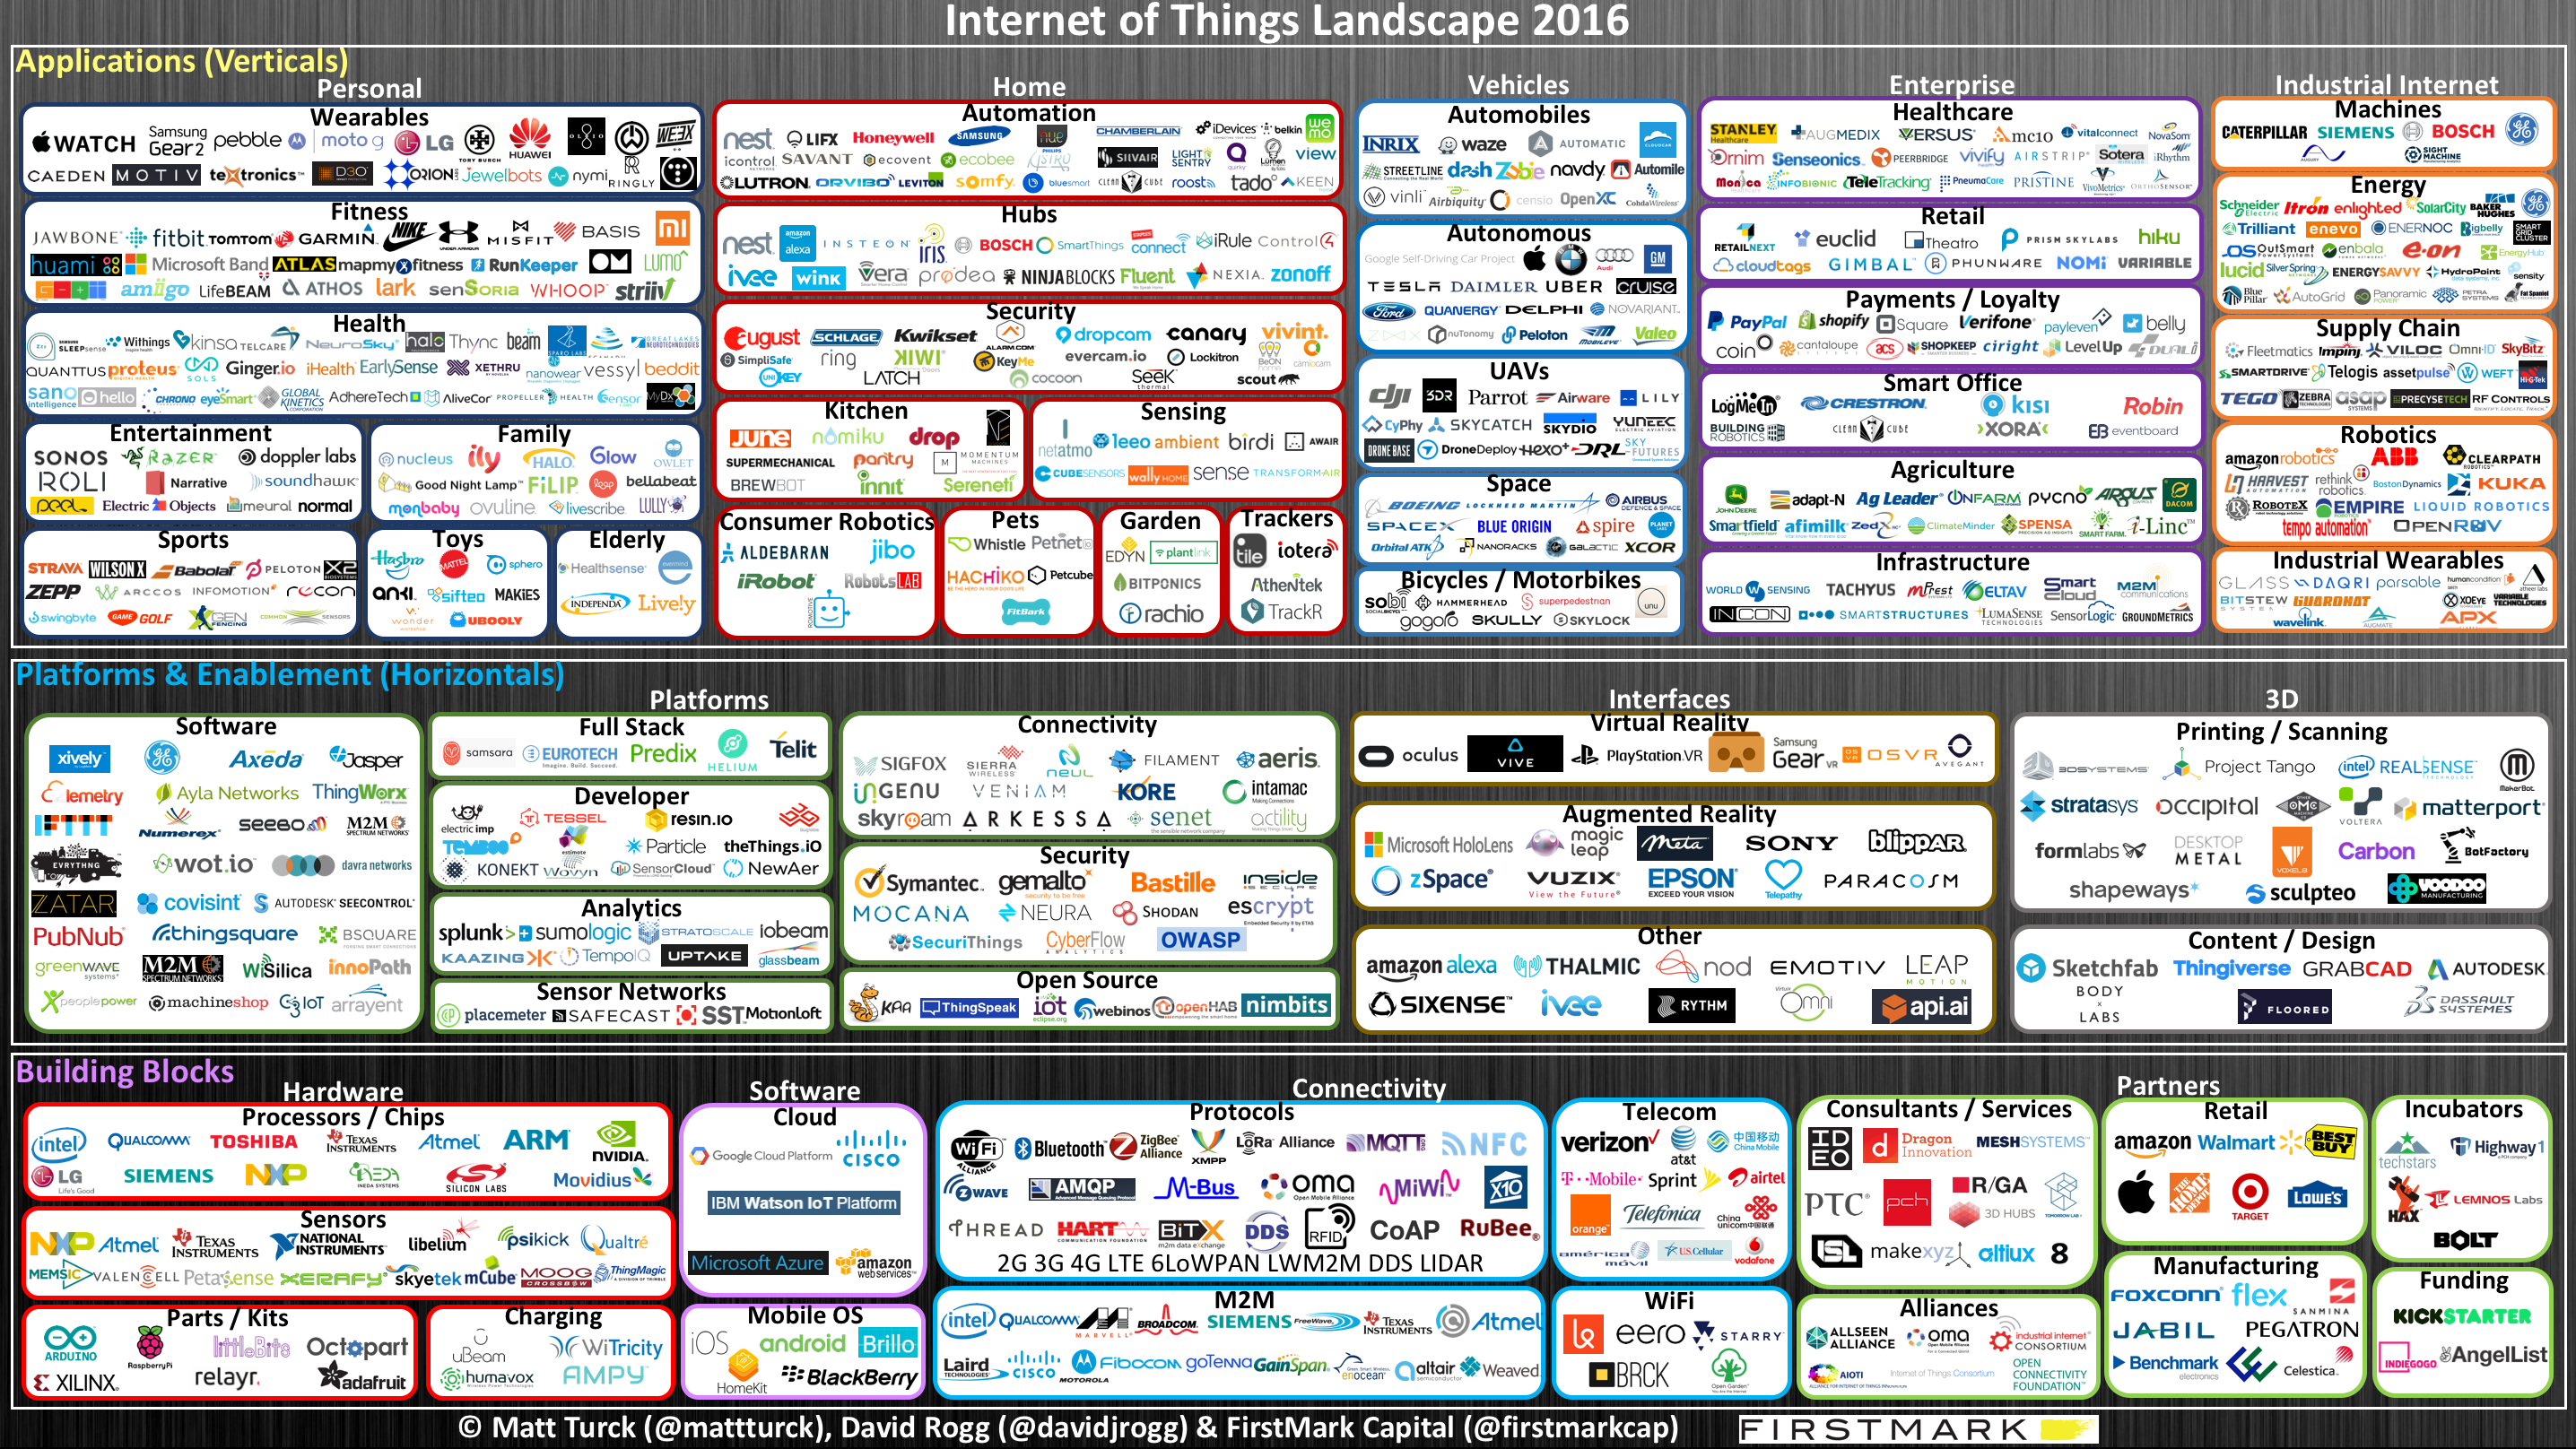
\includegraphics[width=\textwidth]{Figures/IoT-landscape}
\caption[Platforms and Options for the IoT in 2016]{An overwhelming amount of options for consumers and businesses. Source: Matt Turck}
\label{fig:IoT-landscape}
\footnote{http://mattturck.com/2016-iot-landscape/}
\end{figure}


The early Internet was likewise disjointed; accessing files on other computers was often tedious. Each computer connected to the network had a different set of applications, with which users had to be familiar. To counter this Tim Berners Lee invented the Web: the interconnected web of documents accessible in the same way from every computer. The Web revolutionized the way \textit{humans} access documents.


Analogous to the way humans are able to easily access documents all over the world thanks to the Web, so must machines be able to access \textit{data} across devices. However, the autonomous communication and configuration between Things is only possible, when those Things share common information models and implement the same protocols. One proposed approach to this problem reuses established Web technologies, like Semantic Web technology to serve as a common ground. This approach is called the \textit{Web of Things} (WoT). In a sentence its goal is to create a semantic web of data, in which each Thing is represented by a Web resource, which can be queried, much like a database. For this the World Wide Web Consortium (W3C) created a Web of Things Working Group and Interest Group, which together should build the stack for the Web of Things. \cite{.13Nov17}



\section{Motivation -- A Simple Business Case}
To understand the problem at hand, let us first consider the following example. Suppose we are residents of the city of the city of Musterberg, which is planning a cutting-edge water reclamation facility. It should be fully automated and connected to the Internet, so that the reclamation processes can be monitored from afar. This means each sensor and actuator needs a digital representation, which may be stored on one microcontroller.

The city council hires an engineer, Tricia, who must install and configure thousands of sensors and actuators. Aside from the physical configuration, Tricia has to create a distributed system, which could take years. With current technology Tricia would have to configure each device separately and create use cases for interaction patterns. That means, she has to tell devices, with whom they should communicate, what their responsibilities are, and what physical units they are working with.

In the IoT's current state it would require several years of manpower to set up this network and finally would yield a rigid network structure, in which (geographically) mobile Things cannot be easily integrated and additional use cases cannot be easily amended to the system.

Tricia has a deadline of 18 months--Musterberg is experiencing a population boom and the old reclamation facility is projected to not be able to keep up with the demand in within a year and a half. So Tricia has a few options: (1) hire an army of engineers and hope that will solve the problem, (2) use an established IoT platform.

If she (1) hires a large team of engineers Tricia will face the challenge of leading the team, and will certainly require a larger budget, which may not be available. Aside from that, throwing manpower at a problem this complex doesn't always help\footnote{Brook's Law: adding human resources to a late project will make it later.}. If she chooses to (2) use an established IoT platform, she will still likely require additional engineers and have the problem of researching, which platforms provide the services she actually requires. Additionally, most platforms have dubious data policies and confusing pricing schemes. Most platforms won't support the wide range of hardware that the reclamation facility will require, which means multiple platforms may be necessary. This adds the caveat, that they might not be compatible with each other and they also require different programming. This compatibility is referred to as interoperability and is a central challenge the IoT faces.

\begin{comment}


This example shows several of the main challenges the IoT is currently facing:
\begin{itemize}
    \item The difficulty of integrating heterogeneous hardware, this is referred to as interoperability.
    \item The challenge of picking an IoT platform or of using multiple platforms for one system.
    \item The issue of configuring a larger network, so that the system can be running as fast as possible.
    \item Standardization.
\end{itemize}

\change{merge together above and below paragraph}
\end{comment}

The goal of this thesis is to help Tricia by providing two discovery algorithms. One works in a centralized fashion, the other distributed. These algorithms find relevant partners for Things in their network with minimal human interaction. In order to provide proof of concept this work will benchmark the discovery algorithms on a miniature water supply unit from FESTO, which has been outfitted with Web of Things devices. The FESTO device serves as a minimum model for the water reclamation facility.


\section{Contributions}
This work starts by providing a brief background of the technology needed to realize a Web of Things. The focus for this being the importance of Semantic Web technology such as RDF, SPARQL, and the Thing Description.

In the next section the theory behind the three implemented algorithms will be discussed. This includes the REDD algorithm, which is a part of the centralized discovery algorithm, the centralized discovery algorithm itself, and the decentralized discovery algorithm.

After understanding the functionality of the algorithms, the next section will discuss the experimental setup and how the algorithms were evaluated. We will demonstrate the feasibility of discovery algorithms using only established web technology. Here we will also discuss the shortcomings of these algorithms.

This work will then conclude and  give an outlook for semantic discovery in the context of the Web of Things.

\chapter{Related Work}

%- Present state of tech (rather state of the art reports)
%    ==> Comparing theory, like the IoT Survey that's a state of the art reports
%    --> Industry is very interested in the IoT/WoT
%    At present Siemens is not so far; Siemens concentrates on B2B solutions
%- How mature is this technology? --> Technology readiness level for WoT, you make the grade use EU Projects for IoT (hint: there are 7)
%- http://iot-epi.eu/
%- What needs to be done still?
%- Haneberg>> Wissenschaftliche Grundlagen erklaeren? zB: RDF, SPARQL, kurz und bundig erklären, use citation numbers, include in References


This chapter will explain some aspects of one of the most important technologies behind the Web of Things, namely the Semantic Web. A cursory description of the Semantic Web will be provided, the reason it was created, and its role in the Web of Things. We will then discuss two main components of the Semantic Web relevant to this work, RDF and SPARQL and how they relate to a major building block in the Web of Things, the Thing Description. An understanding of these technologies will help when we examine the implemented algorithms.

\section{Interoperability}
A key challenge to the WoT is interoperability, sometimes referred to as integration. The term is used to describe the ability for heterogeneous hardware to seamlessly work together in a network. The mission statement of the W3C for the WoT claims, that the WoT is "intended to enable interoperability across IoT Platforms and application domains" by providing the tools to describe, "IoT interfaces". Through such standards, Things could communicate with one another, regardless of their lower-level implementation or their available networking protocols. \cite{Kazuo.2017}

Experts distinguish between two types of interoperability: vertical and horizontal. Vertical interoperability includes interoperability between hierarchies within one domain, whereas horizontal interoperability allows exchange of data between domains. One can imagine vertical interoperability would be the interoperability of Things within a factory, whereas horizontal interoperability is the compatibility between different factories in a supply chain\cite{wang2016implementing}. The goal of the WoT is to provide both types of interoperability and in this work the discovery algorithms are intended to work in a vertical application.

\begin{figure}[th]
\centering
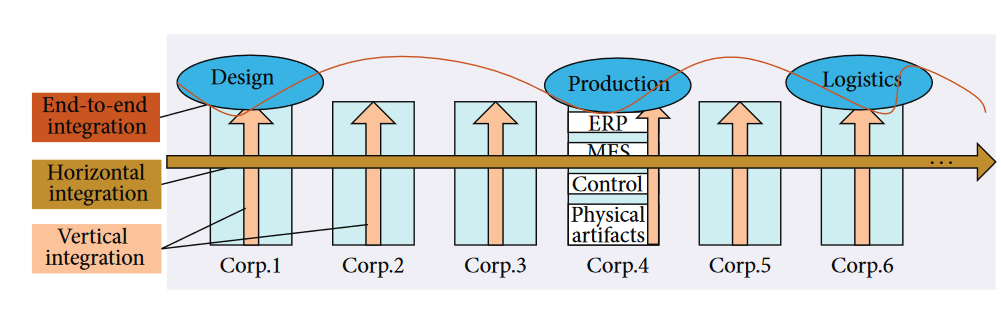
\includegraphics[width=\textwidth]{Figures/integration.png}
\caption{The three types of integration: vertical, horizontal, and end-to-end, as presented in Wang 2016}
\cite{wang2016implementing}
\label{fig:wangIntegration}
\end{figure}

The ultimate goal of the WoT is total horizontal interoperability between different and arbitrarily many domains. By "translating" existing domain standards into machine readable formats instead creating new standards Things can be connected across and within domains\cite{MichahellesWoS}. This combined with Industry 4.0 would mean an exhaustive data exchange between all members of a product's supply chain referred to as \textit{end-to-end} interoperability. This would make products and their respective qualities easily reproducible\cite{wang2016implementing}, thus aiding quality control especially with regards to finding the causes production flaws.

In the example with Tricia and the water reclamation facility, Tricia is charged with designing a system that has vertical interoperability, because she wants to create an integrated smart factory. In an extension of this example, horizontal interoperability would be useful for the integration of the municipal power grid. Let's suppose the reclamation facility has two main power sources aside from the municipal power grid: solar panels and the ability to generate electricity from the decomposing solid waste, raked off before the black water\footnote{waste-water that contains fecal matter.} is processed. It would be useful for the facility to feed power into the gird if there is an abundance of power being generated. Likewise it would help the facility to take advantage of low energy costs, when the municipal grid has a power abundance. As renewable power sources with a stochastic nature, such as wind turbines or solar cells, become more prevalent, this will be more useful, especially since at this scale electricity cannot be effectively stored. Tricia knows this, because she paid attention in her electrical engineering class and is therefore eager to get her plant horizontally integrated.




\section{The Semantic Web}
For the creators of the Web of Things, Dominique D. Guinard and Vlad M. Trifa, it was vital to reuse proven technology to build an architecture for the WoT, rather than develop yet another standard. Guinard and Trifa hoped this would reduce the number of competing standards, thus accelerate the WoT's development. \cite{Guinard.2016} 

The cornerstone of the WoT is the Semantic Web. In the way the Web allows users to easily access documents, so should the Semantic Web allow machines to access data. This is the foundation for machine-to-machine (M2M) communication. In May 2001 Tim Berners Lee first openly discussed the Semantic Web in the \textit{Scientific American}. Its purpose was to extend the Web, so that the information found in it can be easily understood by computers for higher level tasks. Lee proposed an extension to the Web, that was decidedly data-centric for machine consumption, to accompany the document-rich Web for humans. At the time he identified three central components to the Semantic Web: XML, RDF, and ontologies. The first two will be discussed below, the last is a way to link two databases that may use different identifiers to connect the same concepts. For example, look at the zip code. Most US citizens will say ZIP code, elsewhere they may prefer postcode or postal code. How machines should understand that these concepts are all the same is tackled by ontologies. \cite{berners2001semantic}

\begin{figure}[th]
\centering
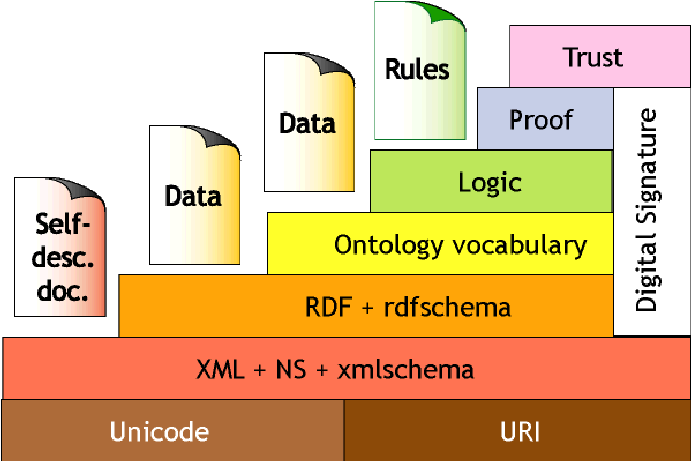
\includegraphics[width=\textwidth]{Figures/SemWebLayer}
\caption{The Semantic Web Layers as Presented by Tim Berners Lee}
\cite{berners2001semantic}
\label{fig:semWebCake}
\end{figure}





Ontologies are a combination of vocabularies and axioms \cite{Cyganiak.2014}. They have vocabularies, taxonomies and inference rules, i.e. a means to define classes and their relationships, and a means to deduce meaning between other ontologies. \cite{berners2001semantic} They can be defined by using the Web Ontology Language (OWL).

The W3C OWL Recommendation defines ontologies as formalized vocabularies with some sort of axiom for describing the nature of relationships. \cite{Synak.2009} \change{this is in the OWL recommendation, not RDF} Ontologies and vocabularies are, to put it curtly, complicated. Semanticists debate their standards and a deep understanding of them surpasses the scope of this work.

In this work the QUDT ontology was used, which describes the relationship between quantities, units, and data types. We only required the vocabularies thereof. The Thing Description is another ontology\cite{Charpenay.2016} this work uses.



%For this work two aspects of the Semantic Web are particularly relevant: RDF for data interchange and SPARQL for querying data.



\section{The Thing Description (TD)}
The Thing Description (TD) is built upon W3C Semantic Web recommendations, specifically the RDF recommendation, which will be discussed in the following section. The success of the WoT depends upon the ability of a Thing to meaningfully expose its capabilities as web resources and interpret the capabilities of other Things\cite{Charpenay.2016}. The TD is currently being drafted and the information is volatile and subject to change, this section refers to the most recently \textit{published} working draft, from April 5, 2018. \change{add this citation, please}


One of these building blocks, the \textit{Thing Description} (TD) standardizes the representation of a Thing's semantic metadata and is analogous the \texttt{index.html} or the landing page of a website. It has not yet been recommended by the W3C, but has only been proposed as a first working draft on September 14, 2017. \cite{Kabisch.2017} \change{add 2018 citation}
Thing Descriptions have been identified as the essential prerequisite for a device to take part in the WoT\cite{Kazuo.2017}. They contain information such as which protocols the Thing supports, which resources and services the Thing has, and where they are, their ids and also names. \change{change citation, TD recommendation}


TDs are serialized by default in JSON-LD, a variant of JavaScript Object Notation, and can either be hosted on the Thing itself or elsewhere, when required. Hosting elsewhere is notably practical when a Thing has limited resources or when legacy devices should be retrofitted to participate in a new WoT system. JSON-LD documents can be serialized in RDF documents due to the mappings between the keywords \texttt{hasThingDescription}, \texttt{hasInteraction}, and \texttt{hasProperty} and \texttt{uris}, \texttt{hrefs}, and \texttt{properties} respectively. The former are contextualized by \url{https://w3c.github.io/wot/w3c-wot-td-context.jsonld}. \change{this can be expanded, love}



Thing Descriptions can be extended by other RDF vocabularies.\cite{Kabisch.2017} In this work the ontology Quantity, Unit, and Data Types (QUDT) \change{this may be confusing, bc above you call it an ontology}\footnote{\url{http://qudt.org/}}, is used to describe the physical units measured like volume and temperature. The ontological model eCl@ssOWL\footnote{\url{http://heppnetz.de/projects/eclassowl/}} was used. ECl@ssOWL was generated from industrial standards and characterizes manufactured products. It enables not only the sensors and actuators to be described, but describes the other physical equipment the system entails. Specifically in the FESTO demonstrator this includes the water tanks and pipes. This work won't go into the details of the used ontologies, because it wasn't especially relevant its contributions and because of the complexity of the ontologies. Here the reader should just know that QUDT is a standard for expressing physical quantities, by standardizing units and ECl@ssOWL allows manufacturers to use\footnote{\uri{www.eclasscontent.com}} standardized metadata for their products. \change{maybe, citation instead of footnote, use sparingly}


\change{Add the TD of the LUT400 here, or snippit of it}

Please note, should the principle behind the TD change, this work assumes that a TD is formalized by an RDF graph and is accessed by an interface based off of the W3C SPARQL recommendation, as is currently intended by the TD developers.



\section{The Resource Description Framework (RDF)}
RDF was first recommended by the W3C on February 10, 2004. As the name implies RDF is a framework used to express information about resources. It serves as a data model to facilitate data exchange on the Web. Similarly to Things, resources include documents, various physical objects, people, or even abstract concepts. When information on the Web needs to be processed RDF can be used, since RDF provides a common framework.

RDF provides a way to extend the linking function of the Web by providing the context of a relationship of a link, and not just a connection between its two ends. Therefore, RDF allows developers to make statements about Web resources. The format of which is a triple with the format \texttt{<subject> <predicate> <object>}. Just like a sentence in a natural language, statements express relationships between two entities, namely the \textbf{subject} and the \textbf{object}. The \textbf{predicate} indicates the nature of their relationship. Relationships are directional and told from the perspective of the subject to the object. A simple example is: \texttt{<Jane> <likes> <Richard> .} Recall that the relationship is directional; this means we know Jane likes Richard, but the triple does not imply that Richard likes Jane. We don’t know about the relationship between Dick and Jane from Richards perspective.

\begin{figure}[th]
\centering
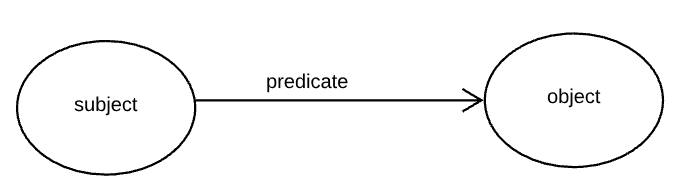
\includegraphics[width=.7\textwidth]{Figures/RDFspo.png}
\caption{RDF data can be represented in graphical form, which is more readable as the data becomes more complex.}
\label{fig:RDFspo}
\end{figure}

Just as sentences can grow in complexity, so can RDF data. It is therefore useful to have different representations of RDF data. Triples, as they appear above can be represented in a graph, which is possibly the simplest mental model. In this model subjects and objects are represented as nodes and the predicates are directed arcs. This is clearly demonstrated in Figure \ref{fig:RDFspo}. A more complicated example of triples is found in Figures \ref{fig:lut400_n-triples} and \ref{fig:rdflut400}, which show the same semantic data from the SITRANS LUT400. They contain elements, that will shortly be explained, but both express exactly the same semantic data for the water level sensor used in the FESTO water management unit. Semantically, there is absolutely no difference between the two, yet the graph is much more readable.


\begin{figure}[ht!]
	\centering
    \fontfamily{pcr}\selectfont
    \begin{tabular}{ l l l }
    <urn:tank1> & <rdf:type> & <ec:C\_AH632010-gen>. \\
    <urn:tank1> & <ex:embeds> & \_:b1. \\
    \_:b1 & <rdf:type> & <ec:C\_AG59007-gen>. \\
    \_:b1 & <wot:hasProperty> & \_:b2. \\
	\_:b2 & <qudt:unit> & <unit:CubicMeter>. \\
	\_:b2 & <qudt:hasQuanityKind> & <quantity:Volume>. \\
	\_:b2 & <wot:hastInteraction> & <coap://192.168.2.61:5683/levelvalue>. \\
	\_:b2 & <rdf:type> & <qudt:Quantity>.
    \end{tabular}

  \caption{Triples from the SITRANS LUT400 water level sensor, which was used in the FESTO Unit.}
  \label{fig:lut400_n-triples}
\end{figure}

So it's clear how RDF data is connected, but not yet clear what the components of an RDF triple are. So what are subjects, objects, and predicates? How can we use them? A resource can be mentioned both as a subject and an object in numerous triples, though not reflexively, e.g. \texttt{<Donald Trump> <loves> <Donald Trump> .} is not allowed.  Subjects, predicates, and objects can be IRIs (Internationalized Resource Identifiers), whereas subjects and objects may be \textit{blank} nodes (more about those in \ref{sec:blanknodes}). Objects may additionally be \textit{literals}, which are used for static values entailing strings, numbers, or dates. Blank nodes, IRIs, and literals are so-called RDF terms. \cite{Cyganiak.2014} 

RDF terms are unique and are not equivalent to each other. For example, the IRI \url{www.zombo.com} is not equivalent to the string literal value of \url{www.zombo.com}, and neither are equivalent to the blank node identifier \url{www.zombo.com} \cite{Cyganiak.2014}.  This is important to note when creating semantic data for a Thing, but in this work semantic data was provided, so it will not be explained in further detail.  \change{this sounds like a cop-out}

An example of a literal can be seen in an extension the LUT400 semantic data as seen in Figure \ref{fig:rdflut400}. In the lower right corner there is the resource \texttt{unit:CubicMeter} from the QUDT ontology, on QUDT page for this resource there is the option to add the abbreviation m\textasciicircum3, which is a \texttt{xsd:string}\footnote{\url{http://www.qudt.org/qudt/owl/1.0.0/unit/Instances.html\#CubicMeter}} and therefore a literal. It would be extended by added an arc with the value \texttt{qudt:abbreviation} and would have the aforementioned literal value.

Ontologies are very similar to RDF, which also describes the relationship between objects, in fact each ontology can be described by an RDF graph. The main difference between the two being: RDF describes the relationship between individual objects and ontologies the nature of relationships between \textit{classes} of objects. \cite{Synak.2009}

\change{Explain the graph}

\begin{figure}[th]
\centering
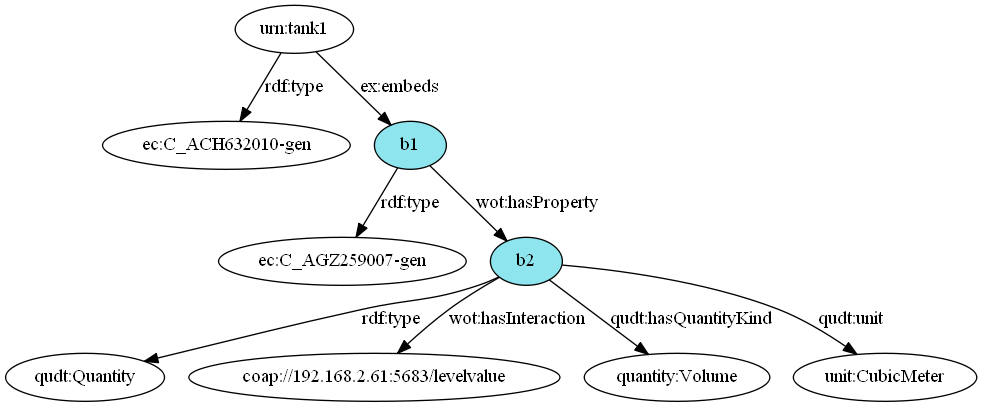
\includegraphics[width=\textwidth]{Figures/lut400}
\caption[The RDF Graph for the LUT400]{RDF Graph of the SITRANS LUT400.}
\label{fig:rdflut400}
\end{figure}


\change{How much information is enough, can additional resources go here?}
\change{Add W3C citation}

\subsection{Blank Nodes}
\label{sec:blanknodes}
Sometimes a node contains neither a resource nor a literal, such nodes are referred to \textit{blank} nodes, sometimes \textit{bnodes}. To see an example of blank nodes, please see Figure \ref{fig:rdflut400}, notice that the blank nodes, in blue, organize the properties of the LUT400 water level sensor and make the RDF graph more readable. Blank nodes can represent complex attributes of other objects\cite{chen2012blank}. E.g. a blank node may be used to organize attributes of an address, which has a postal code, a street name, a city, state/province, a house number, etc. As a part of the RDF standard they represent a core component of the Semantic Web. A 2011 survey found that a majority of the semantic data on the Web contained blank node structures, a minority thereof were complex structures, which are costly to manipulate. \cite{Mallea.2011}

Alarmingly, blank nodes have not been handled consistently by the Semantic Web developers communities; there is a discrepancy between the standard and the implementation. Various serializations of RDF represent blank nodes in unique ways, which makes this problematic for their respective parsers. SPARQL, the query language for RDF regards blank nodes as query variables, which is helpful for the discovery algorithm, since it means that the semantic does not change.

\change{define unlean and connected graphs before this}
\change{blank nodes + OWL = yucky, because when a node has 2 properties, like graphs may be considered unlean in one ontology}
Blank nodes can be problematic: graphs that contain blank nodes and entail joined ontologies may appear unlean, even when it contains no blank nodes. \cite{Hogan.2014} The framework used in this work, Apache Jena, provides methods to compare RDF-graph equivalency. The basis of our this work, requires that graphs do not come from mixed ontologies, because the building of leaned, connected graphs is the foundation of the discovery algorithms. This will be clarified in the next section, where the discovery algorithms are discussed.


\section{RDF Serializations}
RDF describes a graph and as such the representation in computer memory may vary.\cite{Cyganiak.2014} There are many serializations of RDF, but the most common are N-Triples, RDF/XML, and Turtle.


\subsection{N-Triples}
N-Triples is one of the simplest plain-text encodings of an RDF graph. It was originally meant for creating quick RDF test cases, but is now commonly used as an exchange format for RDF data.

N-Triples have a simple subject-predicate-object syntax. RDF IRIs are written in angle brackets and separated by a space, the end of each triple is denoted by a period. Assuming there are no blank nodes in the triple, it would look like this: \texttt{<subject> <predicated> <object> .} Literals are noted by the delimiter \texttt{"} on either side of the literal.

Triples are separated by a new line, which is optional at the end of a document. Comments may be added at the end of each line by using a pound sign (\texttt{\#}). \cite{.02.10.2017c} Looking at N-Triples, it's quite clear why it has become so popular; it has a flat learning curve and it is very quick to generate sample data for testing with.

Figure \ref{fig:lut400_n-triples} shows the LUT400's semantic data written in N-triple format.

\subsection{RDF/XML}

RDF/XML is the format most often associated with RDF, in fact the two are often, incorrectly used interchangeably\cite{Hogan.2014}. The W3C first recommended the serialization in 2004 and then revised their recommendation in 2014\cite{RDFXML.02.10.2017}.

The RDF/XML recommendation defines an XML syntax for RDF graphs to be encoded. Triples can be written a number of ways\cite{RDFXML.02.10.2017}, but basically it works as bellow. Listing \ref{lis:xmlspo} shows the simple s,p,o-triple from figure \ref{fig:RDFspo} in two different RDF/XML notations. The second of which, resemles the format for the LUT400 XML data used in the FESTO unit.

\begin{lstlisting}[language=XML, caption={A trivial RDF triple in RDF/XML}, label={lis:xmlspo}]
<rdf:Description rdf:about="subject">
    <examplenamespace:predicate>
        <rdf:Description rdf:about="object/>
    </examplenamespace:predicate>
</rdf:Description>

<rdf:Description rdf:about="subject">
    <expredicatenamespace:predicate rdf:about="object" />
</rdf:Description>
\end{lstlisting}
\vspace{1cm}

RDF/XML uses Qualified Names (QNames) as its namespace in order to represent IRIs. \change{maybe explain QNames a little more in the RDF section, since this is in common with all serializations}

Compare figures \ref{fig:rdflut400} and \ref{fig:rdfxml}. The first line is like any other XML document, the second is unique to RDF/XML. The graph serialization is typically contained within the \texttt{<rdf:RDF>} and \texttt{</rdf:RDF>} tags. Within the first XML element the namespaces are defined. This works just the same as XML and ensures that there are no naming conflicts. In figure \ref{fig:rdfxml} there are four declared namespaces, which have the prefixes \texttt{demo, qudt, rdf, wot} the first two are needed specifically in the FESTO case. The next element in this figure follows the schema above for the triples and corresponds to \texttt{b1} in figure \ref{fig:rdflut400}. There are two arcs coming out of \texttt{b1}, one goes to \texttt{b2} and is labeled with the predicate names \texttt{wot:hasProperty} and the second points to a web resource with the predicate \textt{rdf:type}. Note that the style of the triple is slightly different in figure \ref{fig:rdfxml} as it is in listing \ref{lis:xmlspo}, this is the same as it would be in normal XML.      \cite{RDFXML.02.10.2017}




\begin{figure}[th]
	\centering
	\resizebox{\textwidth}{!}{\lstinputlisting[language=XML]{Code/lut400.xml}}
    \caption{The LUT400's semantic data represented in RDF/XML format.}
    \label{fig:rdfxml}
\end{figure}


 
Not all RDF graphs can be serialized using the RDF/XML standard, specially those that use the \textt{rdf:HTML} datatype, those that use reserved names as properties, or those that use property names, which cannot be transformed into XML namespace qualified names, e.g. because they contain characters that are not qualified for QName namespaces \cite{RDFXML.02.10.2017}. RDF/XML documents can be validated using a tool\footnote{https://www.w3.org/RDF/Validator/} provided by the W3C.
 
 
\subsection{EXI}
XML is a costly representation of RDF data and embedded devices often do not have the resources to store and process XML. As a result Semantic Web/Linked Data technologies have failed to gain wide-spread traction. To confront this problem researchers at the Siemens Corporate Technology created a solution based off the W3C EXI format. \cite{Kabisch.2015}

The Efficient XML Interchange (EXI) format was formally recommended by the W3C in 2014, and helps to accelerate the exchange of XML data. EXI puts the responsibility of parsing on the server, to which parsing events are sent. It was intended to stream XML data in a without losing any information, unlike RDSZ (The RDF Differential Stream Compressor based on Zlib), with which the RDF structure is lost. This is especially useful when used together with microcontrollers \cite{Kabisch.2015} and when combined with the The Constrained Application Protocol (CoAP) \cite{castellani2011web}. 

As defined in the W3C EXI recommendation, an \textit{EXI stream} "is an EXI header followed by an \textit{EXI body}", which "carries the content of the document, while the EXI header communicates the options used for encoding the EXI body" and is therefore necessary to decode the body. The EXI body is composed of so-called EXI events, which encode XML elements. Below is a list of the EXI events with their descriptions. \cite{.02.10.2017b}


\begin{itemize}

\item \textbf{SD}: Starts the EXI stream with a \textbf{S}tart \textbf{D}ocument event.
\item \textbf{NS}: Sets the \textbf{n}ame\textbf{s}pace of the document.
\item \textbf{SE}: A \textbf{s}tart \textbf{e}lement event, which is used to start the element of an XML document.
\item \textbf{AT}: The \textbf{at}tribute event denotes an attribute in XML. 
\item \textbf{CH}: The \textbf{ch}aracter event denotes a literal.
\item \textbf{EE}: An \textbf{e}nd \textbf{e}lement event, which follows an SE event. This ends the processing of the current element. This event does not refer to the element, like in XML.
\item \textbf{ED}: Ends the document stream with a \textbf{E}nd \textbf{D}ocument event.
\end{itemize}

XML documents can be described using these events. We can again examine this in the semantic data from the LUT400 water level sensor. Looking at listing \ref{lstEXI}, it is easy to see, how the EXI events correspond to the XML data in figure \ref{fig:rdfxml}. These events appear uncompressed, in reality they would be byte compressed in a way similar to Huffman encoding and the namespaces work the same way the QNames work in XML\cite{.02.10.2017b}.



\begin{lstlisting}[caption={The LUT400's XML data as serialized in EXI events.},captionpos=b, label={lstEXI}]
SD
SE	rdf:RDF
NS	xmlns:demo="http://siemens.com/urdf/ns#"
NS	xmlns:qudt="http://qudt.org/schema/qudt#"
NS	xmlns:rdf="http://www.w3.org/1999/02/22-rdf-syntax-ns#"
NS	xmlns:wot="http://w3c.github.io/wot/wot.owl#"
SE	rdf:Description
AT	rdf:nodeID="f8a04ac1a47924de7ad18c3b413895565b1"
SE	wot:hasProperty 
AT	rdf:nodeID="f8a04ac1a47924de7ad18c3b413895565b2"
EE
SE	rdf:type
AT	rdf:resource="http://www.eclass.eu/#C_AGZ259007-gen"
EE
EE
SE	rdf:Description
AT	rdf:nodeID="f8a04ac1a47924de7ad18c3b413895565b2"
SE	wot:hasInteraction
AT	rdf:resource="coap://192.168.2.61:5683/levelvalue"
EE
SE	qudt:unit
AT	rdf:resource="http://qudt.org/vocab/unit#CubicMeter"
EE
SE	qudt:hasQuantityKind
AT	rdf:resource="http://qudt.org/vocab/quantity#Volume"
EE
EE
SE	rdf:Description
AT	rdf:about="http://tank1
SE	rdf:type
AT	rdf:resource="http://www.eclass.eu/#C_ACH632010-gen"
EE
SE	demo:embeds
AT	rdf:nodeID="f8a04ac1a47924de7ad18c3b413895565b1"
EE
EE
EE
ED
\end{lstlisting}



In this work EXI was used to encode semantic data in the XML format. For example, the LUT400's semantic data is 1,098 Bytes in XML vs only XXXXXX in EXI.\change{Size of LUT 400 in EXI}


\subsection{Turtle}
Another syntax for RDF is Turtle: the Terse RDF Triple Language. It is a compact way of expressing RDF and written in an intuitive way. Turtle is compatible with the N-Triples format and the triple pattern specified by the W3C SPARQL recommendation.
\change{are each really written in brackets?}
Like N-Triples, simple triples have the same format: subjects, predicates, and objects are written in that order, each within angled brackets, if they are IRIs. Line comments are also denoted by a \texttt{\#}. Just like in N-Triples, literals are written in quotation marks.

Where Turtle diverges from N-Triples, is in its predicate and object lists. Often the same subjects are referenced in a number of triples. Predicate lists are separated by a semicolon \texttt{;}, whereas object lists are separated by a comma.

\begin{figure}[th]
	\centering
	\begin{lstlisting}[
    basicstyle=\small
]
@prefix rdf:       <http://www.w3.org/1999/02/22-rdf-syntax-ns#> .
@prefix qudt:      <http://qudt.org/schema/qudt#> .
@prefix quantity:  <http://qudt.org/vocab/quantity#> .
@prefix unit:      <http://qudt.org/vocab/unit#> .
@prefix eco:       <http://www.eclass.eu/#> .
@prefix gr:        <http://purl.org/goodrelations/v1#>.
@prefix wot:       <http://w3c.github.io/wot/wot.owl#> .
@prefix demo:      <http://siemens.com/urdf/ns#> .

<http://tank1> a eco:C_ACH632010-gen ; # This is a predicate list
            demo:embeds _:levelsensor .

_:levelsensor a eco:C_AGZ259007-gen ;
              wot:hasProperty _:level .

_:level a qudt:Quantity ;
        wot:hasInteraction <coap://192.168.2.61:5683/levelvalue> ;
        qudt:hasQuantityKind quantity:Volume ;
        qudt:unit unit:CubicMeter .
	\end{lstlisting}
    \caption{The LUT400's semantic data represented in Turtle format}
\end{figure}

Blank nodes in Turtle are denoted by \texttt{\_:} followed by its blank node label.

\cite{Beckett.23.01.2018}

\section{SPARQL}
With RDF semantic data can be represented, but that is nearly useless unless one has a way to query this data.  For example retrieving \url{http://www.munich.de/parking#} could provide data on parking spaces in Munich, which in turn can be identified by their International Resource Identifier (IRI). \cite{Cyganiak.2014} But what really interests someone looking for a parking space is its high-level state: is it free? Does that space include a charging station?


The SPARQL  Protocol and RDF Query Language (SPARQL), pronounced "sparkle", is for querying semantic databases and manipulating RDF data. It was formally recommended by the W3C in 2008  \cite{Herman.2008} and has since been an integral part of the Semantic Web. Tim Berners Lee, the director of the W3C and founder of the Web once said, "Trying to use the Semantic Web without SPARQL is like trying to use a relational database without SQL." \cite{Herman.2008} SPARQL offers tools for querying and analyzing triple patterns and has a similar syntax to SQL. The result of a SPARQL query may be an RDF graph or a result set.
\change{include a sample query of the LUT400, esp one containing blank Nodes}

Again, consider the LUT400. Below is a sample query on the LUT400's data, which selects all triples with the predicate \texttt{wot:hasProperty}.

\begin{lstlisting}[
    basicstyle=\small, caption={A sample SPARQL query on the LUT400's data.}, label={lst:QueryLUT400}]
PREFIX wot: <http://w3c.github.io/wot/wot.owl#>
SELECT *
WHERE {
    ?subject wot:hasProperty ?object .
}
\end{lstlisting}

SPARQL Queries can also be used to compare quantities. Suppose there were two LUT400s built into the FESTO unit, labeled by the simple IDs \texttt{1} and \texttt{2}. The \textt{ASK} command returns either \texttt{TRUE} or \texttt{FALSE} if the query has any matching patterns. The query is formed by asking the web resource of the tank about the property of the water level, and these two results from each web resource is compared.

\begin{lstlisting}[
    basicstyle=\small, caption={Comparing Volume using a SPARQL query}, label={lst:ASKQueryLUT400}]
PREFIX wot: <http://w3c.github.io/wot/wot.owl#>
ASK { 
    <http://example.com/waterlevelsensorID/1> ?wot:hasInteraction ?levelValue1
    <http://example.com/waterlevelsensorID/2> ?wot:hasInteraction ?levelValue2
    FILTER (?levelValue1 > ?levelValue2) .
}

\end{lstlisting}


\cite{.02Oct17}


\change{Allude and Cite Florian Bieringer, his work was important for you!}
\chapter{An Approach to Semantic Discovery}

The backbone of the Web of Things is Semantic Web technology and its clever reuse of established standards to ease the M2M communication, instead of creating novel recommendations. So it makes sense, that the goal of this work is to prove the feasibility of query-based discovery algorithms using only RDF and SPARQL. 

Recall Tricia, who wanted to avoid building a complex vertically integrated system on her own. Now assume she has read a bit about the WoT and would like to apply this to her system. She has TDs for all of the devices, she would like to monitor. That was the easy part, now she has to configure the network and find out which devices should be communicating with one another. The algorithms presented in this chapter will help her achieve this goal with minimal interaction. She understands that the basis of the WoT is to recycle recommendations and to keep her programming as abstract as possible, so she uses the RDF framework and SPARQL to exchange this data.

Both discovery algorithms are based on the consideration that related semantic graphs are necessarily redundant. The proposed discovery algorithms leverage this simple concept by identifying redundant blank nodes in each RDF graph. For example: if NodeMCU 1, which is mapped to the water level sensor wants to affect the water level, it must interact with NodeMCU 3, which controls the valve leading to the same tank.

A third algorithm, which is only used in the centralized discovery algorithm, was implemented. This algorithm runs on a PC client and computes the graph redundancies from two microcontrollers and then sends the leaned RDF graphs back to the microcontrollers.

\section{Graph Theory Refresher}
This work requires some working knowledge of graph theory. There are a few definitions that will be helpful before continuing, including some definitions that are specific to RDF. Listed below are helpful definitions.

\begin{itemize}
    \item A (directed) graph is \textbf{strongly connected} if each node is reachable by following a directed path. If the graph is connected by ignoring path direction, than that graph is \textbf{weakly connected}.
    \item A graph, $G'$ is considered to be a \textbf{proper subgraph} of $G$ if, the group of vertices in the subgraph, $V'$, is a proper subset of $V$ or the edges $E'$ are a proper subset of $E$. Proper in this case means the subset is not equal to the original set. Applied to RDF, a proper subgraph is a proper subset of the triples in an RDF graph.
    \item An \textbf{instance} of an RDF graph is created by replacing some (or all) of it's blank nodes to some set of literals, IRIs, or other blank nodes. Any graph is an instance of itself. Instances are a transitive relation, meaning an instance of an instance of a graph $G$ is also an instance of $G$. \cite{RDFSemantics.Hayes.2014}
    \item An RDF graph is considered \textbf{lean} if there is no instance in a graph, which is a proper subgraph of itself. A non-lean graph contains internal redundancies and expresses the same semantics as their lean subgraph. \cite{RDFSemantics.Hayes.2014}
    \item Two graphs are \textbf{isometric} if, they can be mapped to each other by a 1:1 mapping on their blank nodes. Isometric graphs are treated as being more or less identical, since blank nodes have no identity other than their location in the graph. \cite{RDFSemantics.Hayes.2014}
    \item A \textbf{Connected Subgraph} of a graph $G$ is a subgraph of $G$ containing at least one blank node (as a subject or an object). If a graph contains more than one blank node, then the blank nodes make up a chain, meaning it is possible to navigate through to the next blank nodes by following a directed path until a non-blank node\cite{Esposito.2005}. As an example consider the LUT400 data from figure \ref{fig:rdflut400}, the data starting at \texttt{urn:tank} to the CoAP web resource forms a blank node connected graph; this connected subgraph contains two blank nodes, \texttt{b1} and \texttt{b2}.
\end{itemize}

Here's an example from the W3C\cite{RDFSemantics.Hayes.2014} of an non-lean graph, represented in triples: \newline
\begin{center}
\texttt{ex:a  ex:p  \_:x .} \newline
\texttt{\_:y  ex:p  \_:x .} \newline
\end{center}

Why is this example not lean? If the blank node \texttt{\_:y} were mapped to \texttt{ex:a}, then the triple in the second line would be equal to the first triple. Meaning the instance is a proper subgraph of itself, and therefore is not lean. Now consider following example, also from the W3C\cite{RDFSemantics.Hayes.2014}. Is this graph lean? \newline

\begin{center}
\texttt{ex:a  ex:p  \_:x .} \newline
\texttt{\_:x  ex:p  \_:x .} \newline
\end{center}

Yes, it is lean! There is no mapping for \texttt{\_:x}, which can make the second triple equivalent to the first. Recall, that the reflexive relationship is not allowed, so \texttt{ex:a  ex:p  ex:a .} is not valid, thus \texttt{\_:x} can't be mapped to \texttt{ex:a}.

\section{Implementations}
This section presents three algorithms that were implemented during this case study. The first algorithm culls redundant blank nodes and builds \textit{lean} semantic graphs for the centralized discovery algorithm. The second algorithm discussed will be the centralized discovery algorithm. The final algorithm that will be presented is the decentralized discovery algorithm.


\section{Reducing Redundancies in RDF Graphs}
\label{graphlean}
The previous chapter discussed the W3C RDF recommendation. RDF graphs are a simple way for machines to represent semantic data, but their complexity and size grows explosively as information increases. Therefore, several researchers have put great efforts into reducing the number of blank nodes in an attempt to reduce query times\cite{Esposito.2005}. This is equivalent to computing the \textit{lean} subgraph of the union of all RDF graphs on the network. From the definition of a lean subgraph, it's implied that each non-lean graph has an equivalent and unique lean subgraph\cite{Cyganiak.2014}. In her 2005 paper \textit{REDD: An Algorithm for Redundancy Detection in RDF Models} Floriana Esposito (et al.) \cite{Esposito.2005} created an algorithm with the intention of reducing query times by using this observation to compute lean graphs. Her intention was to reduce query times from graphs that had a large number of blank nodes.



Although the FESTO demonstrator only has five devices attached to it, which are controlled by only three microcontrollers, its combined graph is quite large--the leaned union graph contains twenty blank nodes, whereas the non-lean union contains thirty blank nodes. Figure \ref{fig:festoUnion} shows the core graph of the FESTO demonstrator. The blue nodes are blank nodes and the red nodes are redundant blank nodes. The leaned sum of all of the semantic graphs in the network will be referred to as the \textit{core} of the network. Looking at that significant reduction, it is easy to see the motivation for the REDD algorithm, in fact according to a 2014 survey on blank nodes, about 7.5\% RDF data across all domains were blank nodes\cite{Mallea.2011}.

\begin{sidewaysfigure}
	\centering
	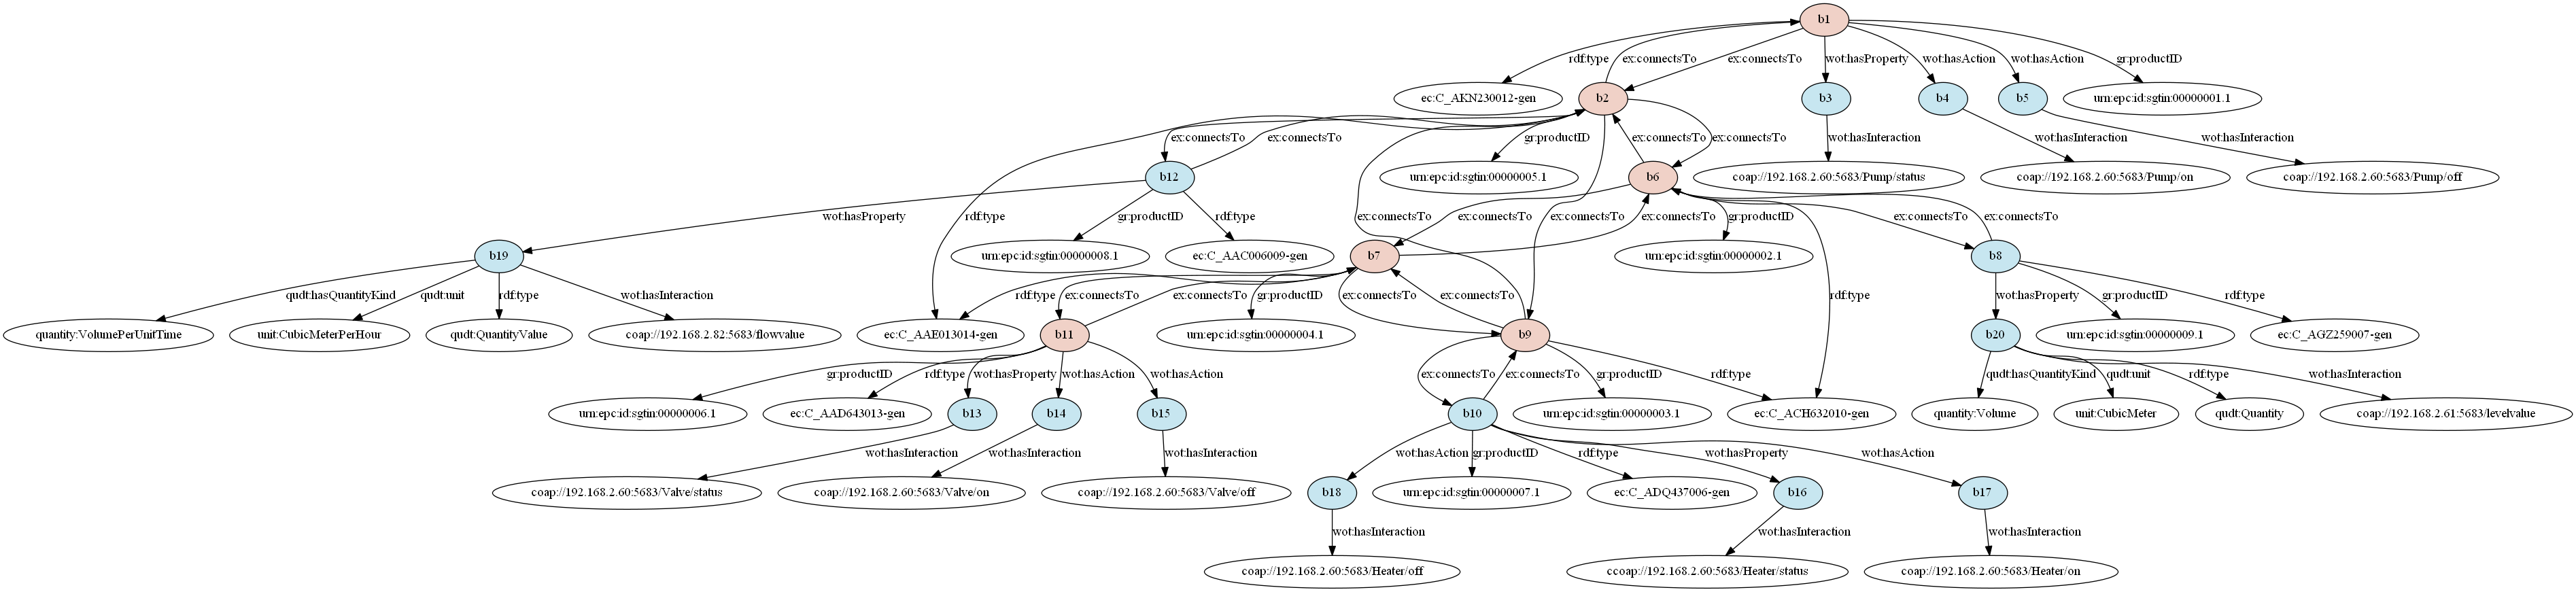
\includegraphics[width=\textwidth]{Figures/RDFUnion.png}
    \caption{Core RDF Graph from the FESTO Demonstrator; the leaned union of all the semantic graphs.}
    \label{fig:festoUnion}
\end{sidewaysfigure}

To do this she started by finding the connected subgraphs within each RDF graph, then taking the created connected graph and converting it to a query, then executing this query against another connected graph from a different set of semantic data. The resultant binding from this query should then be saved in a list and the set of bindings saved as the graph redundancies. Unfortunately, this did not actually reduce query times as much as desired, especially since running the algorithm took so long, but the algorithm presented by Esposito can be leveraged to create the centralized discovery algorithm.

The REDD algorithm proposed by Esposito has three steps: \change{this may be a bit unclear...}
\begin{enumerate}

\item  Build connected graphs from a given RDF graph, $m$
\item Convert each resultant connected graph into a query.
\item  Execute each query against the original graph, $m$.
\item  The set of results are the redundancies in the graph.

\end{enumerate}
Looking closer at the pseudocode in figure \ref{fig:EspositoListing}, we can see she starts by creating a set of connected graphs from one RDF graph in the function declared \texttt{Set CreateConnGraphs(Model m)}. Please note, that she using many of the naming conventions from the Apache Jena library, this library will be discussed in more detail, when we discuss the implementations of these algorithms. Suffice it to say: a model is a just another word for an RDF graph, and a statement is another word for an RDF triple. This means a model is composed of multiple statements, each of which has a subject, predicate, and object.

\texttt{CreateConnGraphs} starts by initializing an empty set for the connected graphs and a map to map the blank nodes to their respective connected graphs. The statements in model \texttt{m} are iterated over. If the statement contains a blank subject then it's checked if that particular "connected" graph is already mapped to that same blank subject, if so the statement is added to the current connected graph. If not a new blank graph is created for the statement and a that new graph is added to the set of connected graphs and the mapping of the blank subject to the connected graph is added to the map \texttt{blanksTocg}. An analogous process occurs for blank objects. \change{should you compare and contrast here?}

\begin{figure}
	\centering
	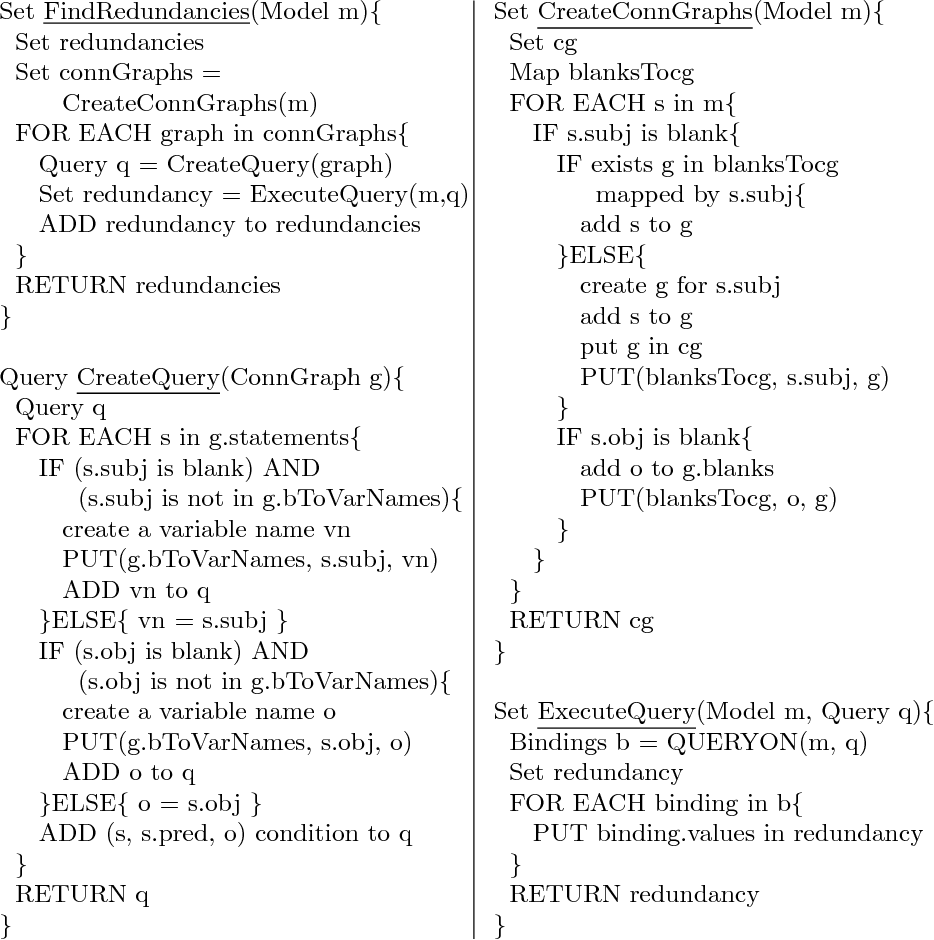
\includegraphics[width=\textwidth]{Figures/REDDlisting.png}
    \caption{The REDD Algorithm as presented in Esposito's 2005 paper.}
    \label{fig:EspositoListing}
\end{figure}

After the connected subgraphs are determined, the algorithm builds queries from the connected graphs in the function \texttt{CreateQuery}. Working through each triple in the connected graph, the query is generated by replacing any blank nodes with query variables. The variable names are come from a map, which as you can see is undefined and unclear, how these were determined. Unfortunately in Apache Jena this is quite a problem and is something that was worked around.

In the third step the queries are executed against the same original model and the query result is added to the set for the redundancies. Executing all of the queries against the original model yields all of the redundancies in the graph. Meaning we find if the original graph can be represented by one of its subgraphs.


The implementation in this thesis followed a similar approach to Esposito. First the algorithm computed the connected graphs in a given RDF graph. These connected graphs are also saved in a set and the blank node mappings to the connected graphs are noted. The connected graphs are then converted to queries, this does not require an extra function as in the Esposito implementation, since a Model can be converted to a query in Apache Jena, then the connected graph queries from the first model are computed against the second model. The same process is then done for the second model to be queried against the first. The algorithm returns a set of RDF node pairs, which are the redundant nodes that will be used by the centralized discovery algorithm.





\lstinputlisting[label={lis:reddPseudo}, caption={The pseudocode implemented in this thesis}]{Code/reddPseudo.txt}
\vspace{1cm}

Finally, the structure of the algorithm was mostly retained, but extended to summarize two RDF graphs contents. How the REDD algorithm was integrated in the centralized discovery algorithm will be discussed in the next section. The details of the REDD algorithm's implementation will be discussed in the next chapter.



\section{Centralized Discovery}
The centralized discovery was used as a baseline. It works by gathering all of the in-network servients' data and executing the \texttt{GraphLean} algorithm locally. The pairs of redundant nodes returned by \texttt{GraphLean} are then used to update each servient's graph, which works as the algorithm below outlines.

The original RDF graph is $G_{i}$, which must be updated in the discovery algorithm. For this two graphs are created: $G^{-}_{i}, G^{+}_{i}$. $G^{-}_{i}$ stores triples that contain redundant blank nodes, which is subtracted from the original graph in order to create $G^{+}_{i}$. Mathematically: $G^{+}_{i} = G^{i}/G^{-}_{i}$. A more precise expression of this update is below:

%For every original RDF graph, $G_{i}$ which should be updated two graphs are created:  The former is used for the redundant blank nodes, the later is the updated graph generated by adding all statements in the difference of . \change{this explanation may be hard to understand}

%This code has been commented out, it is deprecated
\begin{comment}
\change{this has gotten longer, pls change}
\begin{algorithm}
  \caption{Centralized Discovery}\label{centralized}
  \begin{algorithmic}[1]
    \Procedure{Update Servient Graphs}{$G_{1},G_{2}$}\Comment{Update Graph}
    \ForAll{($X_{1}, X_{2}$)} \Comment{$X_{i} \in G_{i}$}
    	\If{$\exists$ Triple $t$ : $t = (X_{1}, $\texttt{wot:hasInterationPattern}, $prop) \in G_{1}$}
      \State $t'\gets (X_{2}, $\texttt{wot:hasInterationPattern}, $prop)$
      \State Add $t'$ to $G_{2}$
      \ForAll{$t$ such that $t = (prop, p, o) \in G_{1}$} \Comment{$o$ is not blank}
      	\State Add $t$ to $G_{2}$
      \EndFor
      \EndIf
    \EndFor \Comment{Repeat with $X_{1}$ and $X_{2}$ swapped}
    \EndProcedure
  \end{algorithmic}
\end{algorithm}
\end{comment}

\begin{enumerate}
    \item Let $G_1, G_2, G^+_1, G^+_2, G^-_1, G^-_2$ be RDF Graphs
    \item For all pairs of RDF nodes ($X_1, X_2$), where $X_1 \in G_1$ and $X_2 \in G_2$,
    \begin{enumerate}
    \item \begin{enumerate}
        \item for all $t \in G_1$ with the form $(X_1, P, O)$,    add $(X_2, P, O)$ to $G^+_2$ and add $t$ to $G^-_1$
        \item for all $t \in G_1$ with the form $(S, P, X_1)$,    add $(S, P, X_2)$ to $G^+_2$ and add $t$ to $G^-_1$
    \end{enumerate} \item \begin{enumerate}
        \item for all $t \in G_2$ with the form $(X_2, P, O)$,    add $(X_1, P, O)$ to $G^+_1$ and add $t$ to $G^-_2$
        \item for all $t \in G_2$ with the form $(S, P, X_2)$,    add $(S, P, X_1)$ to $G^+_1$ and add $t$ to $G^-_2$
    \end{enumerate}

    \end{enumerate}
    
    \item For all $t \in G_1/G^{-}_1$, add $t$ to $G^{+}_{1}$
    \item For all $t \in G_2/G^{-}_2$, add $t$ to $G^{+}_{2}$
\end{enumerate}

The RDF Node pairs, $(X_1, X_2)$ in step 2 are determined by our version of the REDD algorithm. In 2.a the triples from $G_1$ containing the redundant blank node $X_1$ is added to the graph $G^-_1$, the triple containing the other node in this pair is added to the graph $G^+_2$. This occurs in 2.a.i for the redundant blank node as a subject, and in 2.a.ii for the node as an object. 2.b is analogous, but processes triples containing $X_2$. The third and fourth steps add the remainder of the triples that do not contain any redundant blank nodes to their respective graphs. The updated Graphs $G^{+}_{1}$ and $G^{+}_{2}$ are then sent to the servients.

\section{Decentralized Discovery}
The decentralized algorithm is very simple: each device broadcasts one or more queries to the network to which only devices with a non-empty answer should respond. This can be accomplished with just a few lines of code; the broadcasting requires only one line. Though the downfall of this is that there is significantly more overhead, since each servient broadcasts their connected blank node graphs.

For each connected blank node graph $G_i^{b}$ in the RDF graph $G_1$, $G_1^{b}$ should be constructed into a query by replacing the blank nodes in $G^{b}_{1}$ with query variables. This query is then broadcasted to the network. Each device broadcasts as many queries as there are connected blank node graphs in its semantic data. This is similar to the centralized discovery algorithm with the REDD algorithm, where the connected blank node graphs from $G_1$ is queried against the total graph of $G_2$, but each device sends their queries to eat device meaning there are at least $n^2$ as many queries being sent,whereby n is the number of blank node connected graphs in the network, not the number of microcontrollers. \change{maths?}

Upon receiving a broadcast query $G_b^1$ the servient should execute the query against its own RDF graph, $G_{2}$, if the result is non-empty than it should be returned. In this instance the result set is \textit{not} a pair of RDF nodes, but is instead the resultant RDF graph, obtained by replacing all pairs of $(X_1, X_2) (X_i \in G_i), i \in \{1,2\}$ If there is no result, the receiving node should transform the query back into a connected blank node graph and run its own queries against the resultant graph. For the purposes of benchmarking discovery the last step was ignored--the exchange of information was relevant for this work \textit{not} the RDF processing on the microcontroller. It was therefore not implemented and will not specifically be described here.


\change{you first must know how many blank node graphs you have, for this you need a function}
\begin{algorithm}
  \caption{Decentralized Discovery}\label{alg:decentralized}
  \begin{algorithmic}[1]
    \Procedure{Broadcast}{$G_{i}$}\Comment{Send Graph}
    \ForAll{$G^{b}_{i}$  $ \in G_{i}$}
      	\State Convert $G^{b}_{i}$ to a SPARQL query
        \State Broadcast $G^{b}_{i}$
      \EndFor
    \EndProcedure
  \end{algorithmic}
\end{algorithm}
\chapter{Experimental Setup and Evaluation}
\begin{comment}

    Experimental Setup and Evaluation

- Goal of Experiment
- Methods and actual tools used
- Experimental Setup in detail
- Experimental procedure
- Presentation of experimental results

update to overleaf since git is not working!

\end{comment}

This chapter will go over the experimental aspect of this work including the tools and equipment used to implement the algorithms. The setup of the experiments and the testing done on each algorithm and the process of developing these algorithms. The benchmarking results for the two discovery algorithms will be discussed.

We will also present the experimental results for the two algorithms as a proof of concept for the algorithms as presented in the previous chapter.



\section{Equipment and Modeling}
The FESTO water management system was designed for educational purposes in automation. For this work it was equipped with two sensors and three actuators. All of the capabilities of these sensors and actuators are exposed as web resources on three NodeMCU ESP8266 microcontrollers following the Web of Things architecture. Below is the mapping of the microcontrollers to their actuators. In addition to each of the capabilities of their mapped actuators each microcontroller exposes the resources \texttt{/urdfl} and \texttt{/urdfq}, allowing the device to load and query RDF data respectively. In this case the NodeMCU 3 has been mapped multiple devices.

\vspace{1cm}
\begin{figure}[ht]
\centering
\begin{tabular}{l | l}
  water level sensor (LUT400) & NodeMCU 1 \\
  flow sensor (Sitrans F M Mag 6000) & NodeMCU 2 \\
  on/off valve & NodeMCU 3 \\
  pump on/off switch & NodeMCU 3 \\
  water heater on/off switch & NodeMCU 3 \\
\end{tabular}
  \caption{Mappings of Servients to Sensors \& Actuators}
  \label{table:mappings}
\end{figure}

The FESTO unit was originally built as a pedagogical tool to help engineers learn about automation. Here it serves as a minimal viable model of a water reclamation facility. Because the benchmarks only required the semantic data, it was unnecessary to use the FESTO unit while conducting the tests. Instead each experiment was conducted on a with the three NodeMCUs connected to a PC.

\begin{figure}[th]
\centering
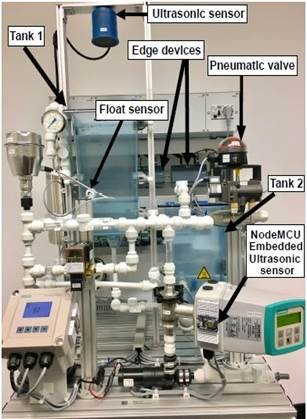
\includegraphics[width=.7\textwidth]{Figures/festoDemonstrator.jpg}
\caption{The FESTO Demonstrator}
\label{fig:festoDem}
\end{figure}



\section{Tools Used}



\subsection{Apache Jena}

Apache Jena is a Java framework used to build Semantic Web applications. It entails various APIs, which work together to process RDF, OWL, and SPARQL. The centralized discovery algorithm required Apache Jena in order to manipulate blank nodes.

There are several modules within Apache Jena, in this paper the most  used was the Core RDF API. In the Core RDF API RDF Graphs can be represented by the data structure \texttt{Model}, which is composed of \texttt{Statements} or may be implemented in the simpler and more limited Java API \texttt{Graph}. \texttt{Statements} entailing one subject, predicate, and object represent a \textit{triple} and are immutable in Jena. This means triple had to be altered when piecing together connected graphs, such as in the \textt{GraphLean} algorithm, the new \textt{Statement}s had to be created with the updated information and the old Statement could then be removed from the \textt{Model} and the new one appended. This process was not included in the benchmarking times, since took place on a PC and the primary interest was the amount of time message passing required. \cite{Jena.24.10.2017}

\subsection{ESP8266}

The ESP8266 is an inexpensive Wi-Fi capable system on a chip (SoC) manufactured by the Chinese company Espressif. It fully supports the TCP/IP stack and 802.11 b/g/n/d/e/i/k/r. The ESP8266 has a small amount of flash memory available--only about 512 kB, though this can be upgraded to 4 MB. The algorithms created in this work were tested using the NodeMCU version of this chip, which includes a special firmware for IoT development. \cite{Zeroday.2017}


This microcontroller is unquestionably rugged: it has an operating temperature range spanning from -40\textdegree{}C to 125\textdegree{}C and is therefore suitable for a wide spectrum of applications. It can be used for home applications, including home automation: monitoring home appliances, monitoring the energy output of photovoltaic cells, managing lights and outlets, baby monitors, etc. It's wide operating temperature range also makes it an appropriate choice in industrial wireless control networks and sensor networks. \cite{espDatasheet} Additionally the ESP8266 has a modest price and is available starting at 5 EUR if purchased individually, with bulk pricing hovering at around 1 EUR per unit. \change{citation needed?}

There are several versions of firmware publicly available for the ESP8266, Siemens created its own version based off of the NodeMCU firmware. A key feature of the NodeMCU firmware is the integration of embedded Lua (eLua) \cite{Zeroday.2017}, which entails the same features as the desktop version plus additional features useful for embedded developers. Like Lua, eLua is able to run on nearly every platform, because it was implemented in ANSI C. \cite{Marinescu.}

Lua is an extensible language, meaning it can integrate functions, which cannot (or should not) be directly written in Lua. This works using the C API, which allows code written in C to interact with Lua. The C API is also available in eLua. The combination of the simplicity and high-level abstraction of a scripting language with the portability and light-weight implementation in C \cite{luaHandbook}, means eLua is powerful tool for embedded developers. This work used Lua in the distributed discovery algorithm.
% https://nodemcu.readthedocs.io/en/master/en/upload/ TODO: continue



\change{removed other picture of NodeMCU, add your own picture of ESP8266, others are copyrighted}

\subsection{ESPlorer}
ESPlorer is an IDE used by ESP8266 developers. It can run on Windows, Linux, MacOS, and Solaris and it provides tools for working in Lua for the NodeMCU and MicroPython. For benchmarking it was run in a virtual machine running Ubuntu 16.04.

\begin{figure}[h]
\centering
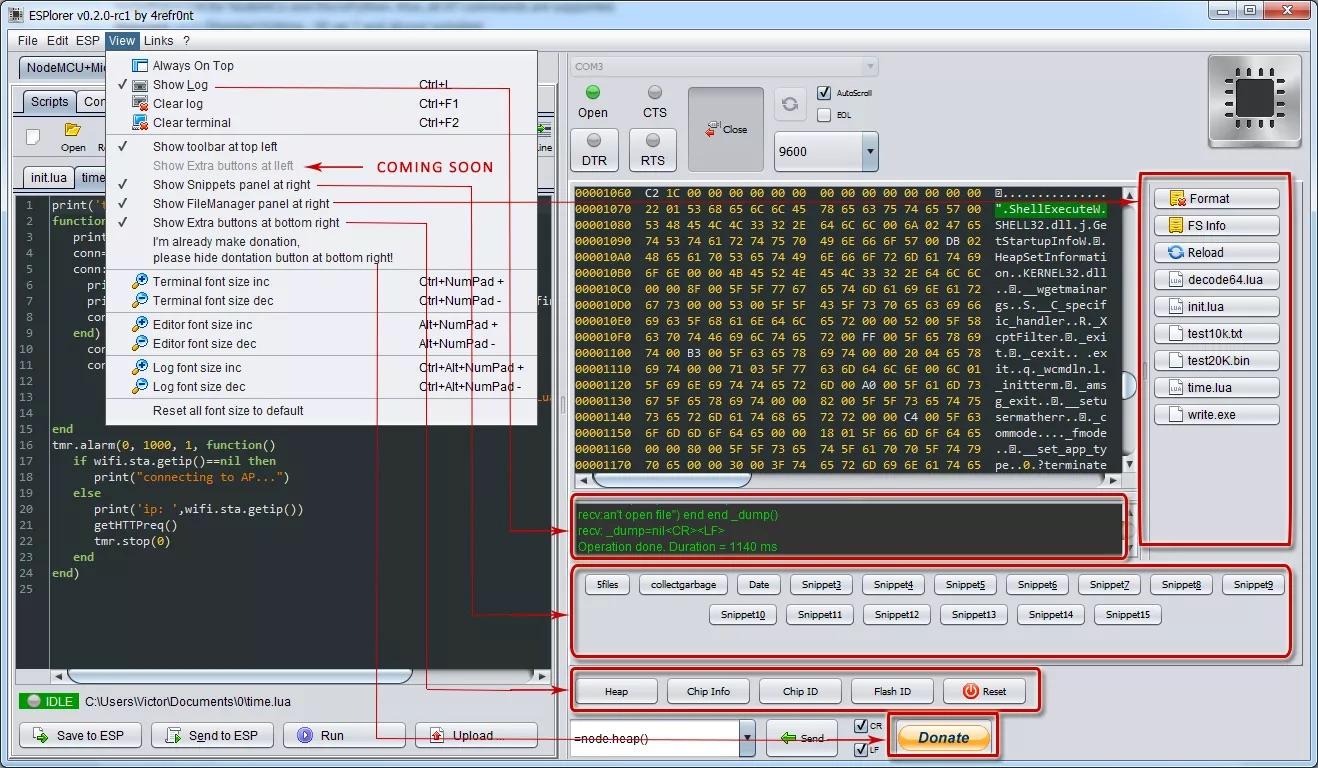
\includegraphics[width=\textwidth]{Figures/ESPlorer.jpg}
\caption{The ESPlorer interface. Image is from the NodeMCU documentation\cite{Zeroday.2017}}
\end{figure}

Code is written in the buffer on the left, while the right buffer shows the current status and connection to the NodeMCU. Connecting to the NodeMCU is simple: after plugging the NodeMCU in, users hit the refresh button in the upper-right corner, then select the COM port, and finally the baud rate.

After a connection to the NodeMCU has been established, code can be simply added and removed from the NodeMCU using buttons in the lower left side of the IDE.

\section{Experimental Procedure}

The modified REDD algorithm was implemented in Java using Apache Jena.

The centralized discovery algorithm also used Jena to compose and send SPARQL queries. \change{come back to this}

This section will outline the implementation details for the algorithm implementations from this work, specifically how they were implemented, how they were tested, and how they were benchmarked.

\subsection{The REDD Algorithm}


The REDD algorithm was vital to the centralized discovery. Since the REDD Algorithm as presented by Esposito et al. was incorrect, we wanted to ensure what we contributed delivered what was intended. Our version of the REDD algorithm was verified by unit testing with JUnit. This includes checking that the queries that were created were created from the models were converted correctly. This was especially important when forming queries containing blank nodes.


Other JUnit tests were created to test the correctness of the algorithms using trivial dummy RDF graphs. This ensured that the resultant blank RDF node pairs computed by the algorithm were in fact correct. Unit tests checked that the blank node connected graphs were created correctly and that the redundant blank node pairs were correct.

Since we had the pseudocode from Esposito (Figure \ref{fig:EspositoListing}), this was used as a framework for our implementation. First the simpler algorithms were implemented, like the \texttt{ExecuteQuery} and the \texttt{BuildConnGraphs} functions. This was estimated to take about two weeks--but ended up requiring more than three months, since the original paper did not contain adequate information to recreate the algorithm and contained definitions from the W3C recommendations used without any further explanation. Other than that the article was vague and even incorrect as submitted, according to one of the paper's co-authors.

Lastly a data type for the connected graphs (\texttt{ConnectedGraph}) was created, as well as a data type for the pairs of \texttt{RDFNode}s, called \texttt{RDFNodePair}.

\begin{figure}[h]
\centering
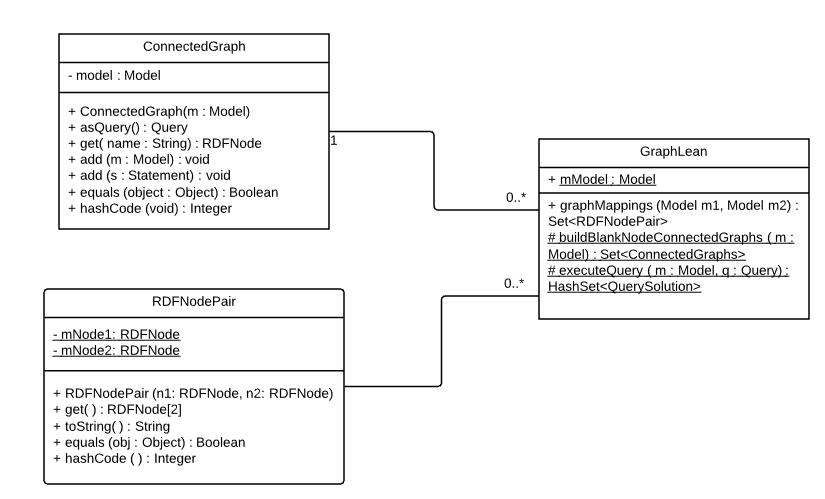
\includegraphics[width=\textwidth]{Figures/REDDuml.png}
\caption{The UML diagram of the implemented REDD Algorithm.}
\end{figure}

We started by implementing the the pseudocode as it was likely intended to be implemented: one graph was processed and searched for redundant subgraphs. As discrepancies came up in the implementation, we reached out to the author, but since the paper was so old (2005), the author no longer had any code and expressed that she neither had the "time, nor the interest" in discussing the algorithm further. So left to our own devices, we rebuilt the algorithm, as we thought was intended and verified using unit testing.

For the tests we created sample data using the Turtle format. like the below, which contains 6 triples and 3 connecte subgraphs. We then tested the \texttt{buildBlankNodeConnectedGraphs} function, by checking that number of blank node connected graphs were correct. This is done in listing \ref{blankNodeJUNIT}.

\begin{lstlisting}[caption={Some sample data that we created for unit testing, written in Turtle.}]
@prefix person: <http://example.com/person/fake/>

person:adam		<p>		_:b3 .
_:b3			<p>		_:b4 .
person:adam		<p>		_:b1 .
_:b1			<p>		_:b2 .
_:b2			<p>		person:bertold .
person:bertold	<p>		_:b5 .
\end{lstlisting}

Listing \ref{blankNodeJUNIT} shows the basic setup of a JUnit Test. The test is marked with a \texttt{@Test} tag before the function declaration. Then an instance of the class to be tested is created. A function was implemented to convert sample Turtle RDF graphs into Jena Models and then the function \texttt{buildBlankNodeConnectedGraphs} was run using the sample model. The actual test is in the last line, where \texttt{assertEquals} checks that the number of connected graphs created by the method is indeed three.

\begin{lstlisting}[language=JAVA, caption={A very trivial test, that checks the correct number of connected graphs in a sample graph is correct for the sample data, in this case sample.ttl contains 3 connected subgraphs.}, label={blankNodeJUNIT}]
@Test
public void buildConnGraphsTest() {
  GraphLean tester = new GraphLean();

  Model m = createSampleModel("sample.ttl");
  Collection<ConnectedGraph> graphs = tester.buildBlankNodeConnectedGraphs(m);
  assertEquals("Number of Conn Graphs must be 3", 3, tester.buildBlankNodeConnectedGraphs(m).size());
}
\end{lstlisting}

This test was run multiple times using different dummy data and each time it worked, so after that the next methods were written. We then moved on to checking if graphs containing blank nodes could be queried without failure.


\begin{lstlisting}[language=JAVA, caption={This test checks if a model containign blank nodes can be queried without returning an error.}]
@Test
	public void blankModelExecutionTest() {
		GraphLean tester = new GraphLean();
		Model m = createSampleModel("sample4.ttl"); // contains no blank nodes
		ConnectedGraph connGraph = new ConnectedGraph(m);
		Model mQueried = createSampleModel("sample5.ttl"); // contains blanks
		Query q = connGraph.asQuery();
		HashSet<QuerySolution> solutions = tester.executeQuery(mQueried, q);

		assertTrue("No solutions found", solutions.size() == 0); // no solutions expected
	}
\end{lstlisting}

Once the REDD algorithm was implemented as it was \textit{most likely} intended in Espoisto's paper, we changed the graph mappings function, to run queries between two graphs: $G_1$ and $G_2$. Finally, this algorithm could be used to update graphs in the centralized discovery algorithm. Each step of the way we ran tests to ensure the algorithm was still functioning correctly.

Our final test took all three NodeMCUs and created the lean subgraph in the network, that all of the NodeMCUs should have. Since this test seen in \ref{lst:coreJUNIT} and all others came back correctly, we continued on to implement the centralized discovery algorithm.

\begin{lstlisting}[language=java, caption={The final test, which checked that the semantic data was being connected, as previously expected.}, label={lst:coreJUNIT}]
@Test
public void findRedundanciesInGraphsTest() {
  GraphLean tester = new GraphLean();

  Model actuators = createSampleModel("actuators.ttl");
  Model lut400 = createSampleModel("lut400.ttl");
  Model pmag = createSampleModel("pmag.ttl");

  Model merged = ModelFactory.createDefaultModel();

  Set<RDFNodePair> redundancies;

  redundancies = tester.graphMappings(actuators, pmag);
  redundancies.addAll(tester.graphMappings(pmag, lut400));
  redundancies.addAll(tester.graphMappings(actuators, lut400));

  merged.add(actuators);
  merged.add(pmag);
  merged.add(lut400);

  List<Statement> toRemove = new ArrayList<>();
  StmtIterator it = merged.listStatements();
  while (it.hasNext()) {
    Statement st = it.next();
    for (RDFNodePair p : redundancies) {
      RDFNode[] array = p.get();
      // take blank node in pair
      RDFNode n = array[0].isAnon() ? array[0] : array[1];
      if (n.equals(st.getSubject()) || n.equals(st.getObject())) {
        toRemove.add(st);
      }
    }
  }
  merged.remove(toRemove);

  Model systemcore = createSampleModel("system-core.ttl");

  assertTrue("Merged Graphs should equal syscore", merged.isIsomorphicWith(systemcore));
}
\end{lstlisting}



\subsection{The Centralized Discovery}

The set-up for the centralized discovery was quite simple: the three NodeMCUs are connected to a PC, which acts as the client.

Each iteration of the centralized discovery can be broken down into two steps: (1) the semantic graphs are combined (2) the resultant lean graphs are sent to the respective servient. Benchmarks measured the time it took for the graphs to be processed with the REDD algorithm and the amount of time it took for the graphs to be sent to the servients, the latter being especially relevant for this work. The former is largely dependent on hardware capability and is not particularly noteworthy.

\change{add activity diagram}

\change{too concise, add more detail}

Between each iteration the times were recorded in a table. \change{expand}


To asses whether the order of the NodeMCUs affected the total time for the discovery algorithm, the benchmark was run ten times with each permutation of the semantic data. Therefore the benchmark ran 60 times in total.



\subsubsection{Results}


\subsection{The Decentralized Discovery}
The decentralized discovery was very simple to implement, but did require the semantic data to be prepared for the algorithm.

The semantic data was converted from the RDF/XML serialization to the EXI format.\change{was also converted to thingy}




The decentralized discovery has a similar setup to the centralized benchmark. All three of the NodeMCUs were connected to a computer. The computer was running a Linux VM. In the VM there were three instances of ESPLorer \change{talk about ESPLorer}

Each NodeMCU was loaded with firmware, which contained a way to store and query RDF data. Each NodeMCU also was loaded with its semantic data in a binary format, Efficient XML, EXI, which was used because requires less broadband and can be processed faster. \cite{} \change{make citation of W3C rec for EXI} \change{EXI is not talked about before, consider discussing in foundations}

In this benchmark there were two quantities we were interested in: the time taken to complete each message pass and the payload size of each message.


\subsubsection{Results}
The original idea of the decentralized discovery was to multicast a query to all nodes. This idea proved to be improbable because of message collisions and timeouts, due to the exposed node problem. \change{flesh me out} Instead of using a multicast IP each NodeMCU had a neighborhood list of the IP addresses in the network and sent queries individual neighbors. In a later implementation, staggering the multicast times on each NodeMCU using a random timer also worked, but rather unreliably. \change{word for one-after-the-other?}


\section{Future Work}

Due to time and scope constraints there are several things that were not accomplished in this work. The REDD algorithm, as implemented here, has quite a few weaknesses regarding blank node management. When we followed up with Luigi Iannone, a co-author of the REDD paper \cite{Esposito.2005}, he recommended another approach using A-Box logic to cull blank nodes. He claimed, that the time savings were not as expected and more importantly that it broke semantic data, when used in datasets with multiple ontologies. This means that the proposed algorithms in this work are not robust.

Regarding the discovery algorithms, the decentralized discovery would be vastly improved if the exposed node problem could be worked around, so that the multicast address could be used in lieu of querying all the neighbors in the neighborhood list. Of course this problem is not just limited to our application, but is a broader problem in wireless sensor networks and ad-hoc systems. By integrating solutions from these frameworks, the decentralized discovery's reliability may be improved. \change{be sure to go into more detail, don't be afraid to write your thoughts on this, pick 1/2 papers and go for it}

The experiment discussed in this paper only examined three microcontrollers, yet scalability is a key challenge to the successful industrial application of these algorithms. Running experiments in scalability will be necessary to have a solid proof of concept. Ideally networks should be tested with 100s or 1000s of nodes. Without suitable hardware simulators, benchmarking this is quite difficult.

In an industrial setting the performance of discovery algorithms applied to mobile devices is especially interesting. For example tracking mobile robots, such as restocking robots, or wearables on employees track of the position of workers on the factory floor, could help to avoid dangerous accidents with heavy machinery. This requires flexible, autonomous reconfiguration of the network. Adding the new device is easier than removing the devices semantic data from the network, so each time the network should remove a device, the web of semantic data would have to be rebuilt from the ground-up. One solution could be taken from relational databases: semantic data that should be deleted could be flagged as inactive, like when an employee leaves after his shift, and then upon arrival in the area his semantic data could be unflagged.

\begin{comment}
--Summary of main part of text
- Deduction made of basis of main body
- Personal opinion of what has been discussed
- Comment about the future
- implications for future work
- important facts and figures not mentioned in body of work
- summary of main points
- concluding Statements
- recommendations
- predictions
- solutions
\end{comment}

\chapter{Conclusion and Outlook}
The aim of this thesis has been to provide proof of concept for discovery algorithms using only fundamental building blocks of the so-called \textit{Web of Things}, with particular emphasis on the industrial application thereof.

A brief overview of relevant Semantic Web technology has been provided.

The central focus of this thesis was the challenge of leveraging Semantic Web technologies, RDF and SPARQL, to create semi-automated discovery algorithms, the feasibility thereof was demonstrated in \ref{chap:experiment}.

In the past year, Siemens along with other researchers have continued to develop W3C recommendations especially Semantic Web recommendations, which will form the backbone of the Web of Things.



%\include{Chapter/preparation}

%----------------------------------------------------------------------------------------
%	THESIS CONTENT - APPENDICES
%----------------------------------------------------------------------------------------

\appendix % Cue to tell LaTeX that the following "chapters" are Appendices

% Include the appendices of the thesis as separate files from the Appendices folder
% Uncomment the lines as you write the Appendices

%\include{Appendices/AppendixB}
%\include{Appendices/AppendixC}

%----------------------------------------------------------------------------------------
%	BIBLIOGRAPHY
%----------------------------------------------------------------------------------------

\printbibliography[heading=bibintoc]

%----------------------------------------------------------------------------------------

\end{document}
